




% SHIFT v1 (revision 2, 2026-11-18). Recent literature re-checked online 2026-11-18.
% Observed results: results/processed/rq1/rq1_summary.json, rq1_paired.csv,
%   results/processed/rq234/{summary.json,patches.csv,units.csv},
%   results/processed/revision/{revision_stats.json,exhaustive_audit.json,*.csv},
%   results/raw/revision/exhaustive_followup/*.json (31 + 7 follow-up executions).
% Figures between %<<GEN:...>> markers are generated by analysis/revision/figures.py --inline.
% The DSL frontend and review gate are proposed, not evaluated implementations.
% 20 X units are excluded from conclusive-label denominators.
% Build outside this directory to preserve the two-file deliverable.
\documentclass[a4paper,fleqn]{cas-sc}
\usepackage[T1]{fontenc}
\usepackage[authoryear,round]{natbib}
\usepackage{amsmath,amssymb,amsthm,algorithm,algpseudocode}
\usepackage{array,booktabs,tabularx,listings,xcolor,tikz,graphicx,placeins}
\usepackage{pgfplots}
\usepackage{placeins}
\usepackage{float}
\pgfplotsset{compat=1.18}
\usepgfplotslibrary{statistics}
\usetikzlibrary{positioning,arrows.meta,calc}
\definecolor{okblue}{HTML}{0072B2}\definecolor{okorange}{HTML}{E69F00}
\definecolor{okverm}{HTML}{D55E00}\definecolor{okgrey}{HTML}{999999}
\hypersetup{hypertexnames=false,hidelinks}
\newcommand{\tool}{\textsc{Shift}}
\newcommand{\dsl}{\textsc{Shift-Intent}}
\newcommand{\code}[1]{\texttt{\detokenize{#1}}}
\newcommand{\lab}[1]{\textsf{#1}}
\newcommand{\cl}{\operatorname{cl}}
\newcommand{\withdraw}{\operatorname{withdraw}}
\newcommand{\Valid}{\operatorname{Valid}}
\newtheorem{definition}{Definition}
\newtheorem{proposition}{Proposition}
\lstset{basicstyle=\ttfamily\footnotesize,columns=fullflexible,keepspaces=true,
  breaklines=true,frame=single,numbers=left,numberstyle=\tiny,numbersep=7pt,
  xleftmargin=1.5em,showstringspaces=false,tabsize=4}
\renewcommand{\topfraction}{.95}
\renewcommand{\bottomfraction}{.9}
\renewcommand{\textfraction}{.05}
\setcounter{topnumber}{3}
\setcounter{bottomnumber}{2}
\setcounter{totalnumber}{5}
\begin{document}
\let\WriteBookmarks\relax
\shorttitle{Behavioral Contracts for Agent-Generated Patches}
\shortauthors{Babaei}
\title[mode=title]{SHIFT: Governing Agent-Generated Patches through Behavioral Contracts and Counterfactual Change Analysis}
\author[1]{Majid Babaei}[orcid=0000-0002-1394-4030]
\cormark[1]
\ead{majid.babaei@ufv.ca}
\affiliation[1]{organization={School of Computing, University of the Fraser Valley}}
\cortext[1]{Corresponding author.}

\begin{abstract}
AI coding agents increasingly automate software repair, yet their final patches may contain edits that contribute little to the intended fix or preserve remnants of unsuccessful repair attempts. Existing change impact analysis identifies potentially affected program elements but does not establish whether individual edits are necessary to achieve the desired behavior while preserving existing functionality. This distinction motivates a fundamental question: how can the contribution of each edit be established without assuming that a valid repair must follow a particular implementation path? We introduce \tool{}, a contract-driven approach that evaluates patch contributions through dependency-aware counterfactual execution. \tool{} formalizes repair goals and preservation obligations as behavioral contracts, systematically evaluates edit withdrawals, identifies a passing reduced patch, and assigns contextual roles to edits based on executable evidence. It further investigates potential regressions through targeted additional testing. We also implement \dsl{}, a declarative language for specifying behavioral contracts, and compile contracts with it for every evaluated task. Its benefits for contract authors remain to be evaluated with users. We evaluate \tool{} on SWE-bench Verified, analyzing 22,954 agent patches from 46 model systems and conducting counterfactual experiments on 1,674 agent and reference patches. Our findings challenge the assumption that agent-generated patches are systematically broader than human repairs and reveal that approximately one-third of source edits in both groups can be removed without violating the evaluated behavioral obligations. Moreover, location-based analysis overlooks most removable edits, while \tool{} provides executable evidence of edit contributions, identifies reduced patches of minimum size under its dependency relation in all but one exhaustively checked case, and improves regression detection through additional testing. A trajectory-free reimplementation of the closest prior minimizer is cheaper on large patches and agrees on most witnesses; where the two disagree, the disagreements expose limitations of both. These results highlight the importance of behavior-based, rather than location-based, assessment for both AI-generated and human-written patches.



%We evaluate \tool{} on SWE-bench Verified through a footprint analysis of 22,954 agent patches from 46 model systems and an execution-based study of 1,379 resolved agent patches and 295 reference patches. Contrary to the assumption that agent-generated repairs are systematically broader, no directional footprint difference satisfies our prespecified cross-system criterion. Under the benchmark's behavioral obligations, 34.1\% of conclusively classified agent source edits and 35.9\% of reference source edits are removable, with substantial variation across systems. Reference-file overlap fails to identify 72.9\% of removable agent edits, demonstrating the limitations of location-based relevance judgments. Additional tests increase semantic mutation detection from 31.3\% to 41.4\%, while the reduced witnesses achieve minimum cardinality in 1,602 of 1,603 small patches under exhaustive verification. These findings establish that edit-level contribution cannot reliably be inferred from patch size, location, or authorship alone. Instead, behavioral contracts and executable counterfactual evidence provide a principled foundation for assessing both agent-generated and human-written repairs.
\end{abstract}
\begin{keywords}
agentic software engineering \sep change impact analysis \sep behavioral contracts \sep counterfactual analysis \sep delta debugging \sep program repair \sep patch review
\end{keywords}
\maketitle
\raggedbottom

% \section{Introduction}\label{sec:introduction}

% When a coding agent submits a patch, a maintainer must decide more than whether the reported bug has disappeared. The maintainer must also decide whether the other changes belong in the repair, whether they alter behavior that should remain stable, and what evidence justifies keeping them. Repository-level agents inspect code, revise hypotheses, edit several modules, and execute tests before producing a single patch~\citep{yang2024sweagent,bouzenia2025trajectories}. The final diff compresses that process. An apparently coherent change can therefore contain both the successful repair and remnants of other attempts. Accepting all of those edits increases the code that reviewers must understand and that future developers must maintain. Rejecting unfamiliar edits can instead discard a valid repair that takes a different route from the maintainer's own solution.

% Recent work documents such residual changes. TRIM reports that agent-generated patches tend to be larger than the corresponding human implementations and removes search leftovers by counterfactual execution guided by agent trajectories~\citep{mathai2026trim}. SlopCodeBench reports growing verbosity and structural erosion when agents repeatedly extend their own code~\citep{orlanski2026slopcodebench}. These studies motivate an examination of agent artifacts. They do not establish that every agent patch is broader than a human one, and their measurements depend on scaffolds and tasks. We therefore treat a human--agent difference as a hypothesis to test rather than a premise.

% Existing analyses answer related but different questions. Change impact analysis (CIA) starts from modified statements, functions, or files and estimates what they may affect~\citep{bohner1996cia,li2013cia}. Regression test selection uses such dependencies to decide which tests to rerun~\citep{rothermel1997safe,gligoric2015ekstazi}. These techniques apply to human and agent changes alike. Here the limitation is the question they answer, not an assumption about the author. Knowing that a branch affects a test does not establish that the requested repair needs the branch. Overlap with a reference patch shows where one developer repaired a defect, not every location where a valid alternative could be implemented. Patch correctness assessment asks whether a passing patch generalizes beyond its tests~\citep{qi2015kali,smith2015cure}, but does not explain the role of each constituent edit. Delta debugging and TRIM find smaller passing configurations~\citep{zeller2002ddmin,mathai2026trim}. A smaller passing patch alone does not tell a reviewer which edits failed when withdrawn individually, which ones were omitted only together with others, or whether the omitted edits change behavior beyond the tests that were used.

% Consider a Django issue in which a lazily wrapped URL argument causes a database query to fail. The maintainer repairs the view that creates the wrapper. An agent instead adds unwrapping logic in two database modules. The agent patch passes the issue's goal test and 52 preservation tests, but only the edits in one of those modules are required for those outcomes. Every agent edit lies outside the maintainer's reference file. Location alone therefore treats the useful and the removable route alike, and whole-patch acceptance keeps both. Section~\ref{sec:running} presents this recorded case as the running example.

% We address the following problem: \emph{given a candidate repair and explicit behavioral obligations, how can a reviewer establish which groups of edits support the observed repair, which can be omitted, and which are implicated in observed preservation failures?} Our central insight is that relevance should be defined relative to a stated behavioral contract, not relative to a reference location. Edit locations remain necessary for constructing program variants and selecting additional tests, but they do not define relevance. This choice admits alternative repair routes while requiring evidence for the changes that accompany them.

% \tool{} links a behavioral contract to executable counterfactuals. The contract separates behavior to achieve from behavior to preserve. The analysis decomposes the patch and records dependencies between edits, so that a withdrawal does not leave an added use without its definition. It then combines withdrawal experiments with dependency-aware reduction to find a passing subset and classifies each edit relative to it. Finally, a preservation envelope selects additional tests and uses add-back experiments to associate observed regressions with omitted groups. Each conclusion carries a witness configuration and a recorded outcome. A proposed contract language, \dsl{}, gives these obligations a reviewable textual form. Its parser and review gate are designs, not evaluated components.

% The evaluation tests the motivating premise as well as the technique. Across 46 systems using the mini-swe-agent scaffold family, agent patches tend to be smaller and less dispersed than reference patches, but no directional difference meets the two-thirds-of-systems criterion fixed in our protocol. Among conclusively classified source edits of 1,379 resolved agent patches, 34.1\% can be omitted while preserving the benchmark obligations. The proportion for reference patches is 35.9\%, and individual systems range from 9.7 points below to 19.3 points above their matched reference patches. The need for edit-level evidence is therefore neither unique to agents nor explained by patch size. The envelope detects additional mutation probes, while most remain undetected. An audit of the reduction results located and corrected a defect in the exhaustive-search baseline. After the correction, the witness has minimum cardinality in all but one of 1,603 small patches.

% The paper makes three contributions:
% \begin{enumerate}
% \item \emph{A contract-relative formulation of edit contribution.} It separates goal obligations, preservation obligations, and supplementary envelope observations. It defines dependency-closed withdrawals and four operational edit roles. A proposed textual form, \dsl{}, comes with its syntax, static checks, and execution semantics. The parts that remain unimplemented are stated.
% \item \emph{A counterfactual analysis with stated guarantees.} The analysis returns a passing witness with withdrawal minimality under explicit oracle assumptions, an omission witness for every removed edit, and add-back associations for envelope regressions.
% \item \emph{An empirical assessment on SWE-bench Verified.} It covers footprints across 46 systems, edit roles for 1,674 executed patches with matched agent--reference comparisons, location and LLM-judge approximations, mutation-based preservation probes, cost, and an audited minimality comparison. A protocol for the unevaluated parts of the workflow completes the assessment.
% \end{enumerate}

% Section~\ref{sec:background} introduces the concepts and running example. Section~\ref{sec:approach} presents the architecture and method. Section~\ref{sec:evaluation} reports the evidence, discusses it, and specifies the remaining studies. Section~\ref{sec:related} compares the approach with the closest research families.






\section{Introduction}\label{sec:introduction}

A coding agent can fix a reported bug and still submit changes that the fix does not need. A passing test suite establishes that the patch satisfies the tested requirements, but it does not explain why each edit belongs in the patch. This distinction matters when agents explore alternative fixes, modify several parts of a repository, and consolidate their work into a final diff~\citep{yang2024sweagent,bouzenia2025trajectories,mathai2026trim}. A maintainer must then decide whether to retain all changes, remove seemingly unrelated ones, or request another repair. Making these decisions requires evidence of what individual edits contribute to the intended fix.

The problem is not unique to AI-generated code. Previous studies have shown that changesets can mix distinct development concerns, making them harder to review and analyze~\citep{herzig2013tangled,barnett2015untangle}. More recently, TRIM identified residual changes in agent-generated repairs and used execution evidence from agent trajectories to remove them~\citep{mathai2026trim}. SlopCodeBench further examined how code quality can deteriorate during repeated agent-driven development~\citep{orlanski2026slopcodebench}. Although these findings raise concerns about agent-generated patches, they do not establish that such patches are generally less focused than human-written repairs. Determining whether this difference exists requires comparisons across matched tasks and agent systems.

The main challenge is that existing techniques do not directly establish which edits contribute to a successful repair. Change impact analysis identifies program elements and tests potentially affected by a modification~\citep{li2013cia,ren2004chianti}. However, an edit may affect a test without being necessary for it to pass. Patch correctness assessment examines whether a test-passing repair is likely to be correct~\citep{qi2015kali,smith2015cure,wang2020apr}, but even a correct patch may contain unnecessary changes. Delta debugging identifies smaller configurations that preserve an observed outcome~\citep{zeller2002ddmin}. Nevertheless, finding a smaller passing patch does not fully explain the contributions of interacting edits or reveal preservation failures beyond the tests used for reduction. Furthermore, because tests provide only partial specifications of intended behavior~\citep{barr2015oracle}, removing an edit without causing test failures does not establish that the edit is harmless in every context. These limitations highlight the need for an analysis that relates individual edits to explicit behavioral requirements and supports its conclusions with reproducible execution evidence.

To address this problem, we introduce \tool{}, an approach for assessing edit contributions against a \emph{behavioral contract} that specifies what a repair must achieve and which existing behaviors it must preserve. Instead of relying on similarity to a reference patch, \tool{} evaluates the consequences of withdrawing individual edits and groups of dependent edits. It first decomposes a candidate patch into edit units and identifies dependencies required to construct meaningful program variants. It then executes counterfactual tests to identify a smaller passing patch and characterize the contribution of each edit relative to the resulting witness and full-patch withdrawal outcomes. To investigate possible regressions, \tool{} selects additional preservation tests and performs add-back experiments on omitted edits. The resulting evidence supports edit-level review decisions, although its conclusions remain limited to the evaluated behavioral obligations rather than unrestricted semantic equivalence. We also provide \dsl{}, a textual notation for expressing behavioral contracts, with a parser, static checks, and baseline validation. Its usability for contract authors is outside the scope of the present study.

We evaluate \tool{} using SWE-bench Verified~\citep{jimenez2024swebench,chowdhury2024verified}. First, we compare 22,954 agent-generated patches from 46 model systems with reference repairs to investigate differences in their change footprints. We then conduct execution-based counterfactual analyses on 1,379 resolved agent patches and 295 reference patches. Contrary to the assumption that agent-generated patches are consistently broader, no directional footprint difference satisfies our prespecified cross-system criterion. Nevertheless, our analysis identifies removable source edits in both groups. Specifically, 34.1\% of conclusively classified agent edits and 35.9\% of reference edits can be omitted while preserving the evaluated obligations. We also find that reference-file overlap fails to identify 72.9\% of removable agent edits, demonstrating the limitations of location-based relevance judgments. Additional preservation testing improves mutation-probe detection, although substantial gaps remain. An exhaustive audit confirms that the reduced patches achieve minimum cardinality among dependency-closed configurations in 1,602 of 1,603 small cases. A diff-only reimplementation of TRIM's search costs less on large patches and returns the same witness in 94\% of patches. Its smaller witnesses mostly reveal an over-approximating dependency relation in \tool{}. Finally, the contract language reproduces the study's obligations for all 295 tasks, and its baseline check flags nine benchmark contracts that the base revision does not meet. These findings show that edit-level assessment is relevant to both agent-generated and human-written repairs and that removability under a behavioral contract should not be confused with universal redundancy.

This paper makes three contributions:
\begin{enumerate}
\item \emph{A contract-relative formulation of edit contribution.} We distinguish repair goals from preservation obligations and define dependency-aware withdrawals and contextual edit roles without assuming a unique correct implementation. The \dsl{} language and its frontend make these contracts explicit, statically checked, and executable.
\item \emph{An executable counterfactual analysis.} \tool{} identifies a passing reduced patch, records execution evidence for retained and omitted edits, and investigates observed preservation failures using additional tests and add-back experiments. We also establish the conditions under which its reduction guarantees hold.
\item \emph{An empirical study of patch contributions.} We investigate patch footprints, edit removability, the limitations of reference-location judgments, preservation-test sensitivity, and reduction quality across agent-generated and reference repairs.
\end{enumerate}

Section~\ref{sec:background} introduces the necessary concepts and running example. Section~\ref{sec:approach} describes \tool{} and its underlying methodology. Section~\ref{sec:evaluation} presents the experimental evaluation and discusses the findings. Finally, Section~\ref{sec:related} reviews related work.


%=====


% \section{Background and problem formulation}\label{sec:background}

% \subsection{Agentic repair and executable task outcomes}\label{sec:agents}

% A repository-level coding agent receives an issue and a base revision, interacts with development tools, and returns a patch. Its scaffold determines the available actions, feedback, and stopping rules. The model and scaffold together constitute the evaluated system. Differences between systems can therefore arise from model capability, prompting, tools, patch extraction, or execution policy. Observing a final patch does not separate these causes.

% SWE-bench represents repair tasks using real issues, base revisions, reference patches, and test specifications~\citep{jimenez2024swebench}. SWE-bench Verified is a human-screened subset of 500 instances~\citep{chowdhury2024verified}. Its \code{FAIL_TO_PASS} tests fail on the base and should pass after the repair. Its \code{PASS_TO_PASS} tests encode previously passing behavior that should remain passing. An instance is resolved when both sets pass. This criterion makes repair outcomes executable, but it measures selected tests rather than all intended behavior.

% A reference patch is useful for reconstructing an environment and comparing repair locations. It is not a unique correct solution or a minimal specification. We distinguish \emph{agreement with the reference route}, \emph{passing the benchmark obligations}, and \emph{correctness beyond those obligations}. The approach targets the second and gathers additional, necessarily incomplete evidence about the third.

% \subsection{Impact, fault localization, and reduction}\label{sec:foundations}

% CIA estimates the consequences of a modification through static or dynamic dependencies~\citep{li2013cia,orso2003field}. Chianti, for example, decomposes changes and relates them to affected tests~\citep{ren2004chianti}. Fault localization instead ranks program elements according to their association with a failure~\citep{wong2016fl}. Both can inform repair, but neither relation is identical to the contribution of an edit in an already passing candidate. A suspicious location may admit several alternative repairs. A changed element may influence a test without being required for that test to pass.

% Delta debugging isolates a smaller set of changes that retains an outcome of interest~\citep{zeller1999yesterday,zeller2002ddmin}. Here that outcome is success under obligations, rather than a failure. Structure-aware reduction can avoid some ill-formed configurations~\citep{misherghi2006hdd}. Dependency-aware reduction must additionally distinguish a failed behavioral experiment from an invalid program variant.

% Three notions of smallness must remain separate. A configuration is \emph{withdrawal-minimal} if no permitted elementary withdrawal preserves success. It is \emph{inclusion-minimal} if no proper subset succeeds. It has \emph{minimum cardinality} if no successful configuration has fewer units. Without assumptions on how outcomes vary with subsets, the first implies neither of the other two. Compensating edits can make each individual removal fail even though removing both succeeds. \tool{} guarantees only withdrawal minimality under the assumptions in Section~\ref{sec:triage}. Section~\ref{sec:rq4} measures how often minimum cardinality is also attained.

% \subsection{Behavioral contracts and the observation boundary}\label{sec:contracts}

% An edit's contribution is meaningful only relative to a requirement. We therefore make the executable obligations explicit before defining edit roles. This follows the contract principle of stating required behavior~\citep{meyer1992dbc}, while recognizing that a test suite is a partial specification~\citep{barr2015oracle}.

% \begin{definition}[Behavioral contract]\label{def:contract}
% For a base revision $P$, a behavioral contract is $K=(T_g,T_p,\eta,\rho)$, where $T_g$ is a nonempty set of goal tests, $T_p$ is a set of preservation tests, $\eta$ is a preservation-envelope selection policy, and $\rho$ specifies repeated execution and unknown-outcome handling. The core obligations are $T_g\cup T_p$. The envelope supplies additional observations and is reported separately.
% \end{definition}

% Separating the envelope from the core prevents a silent change in the meaning of a label. A unit can be removable for the core obligations and still participate in an envelope regression. Adding an independently justified preservation test to $T_p$ creates a new contract and requires a new analysis. It does not retroactively change what an earlier run established.

% Execution can produce a test failure, an ill-formed variant, or missing evidence, and each needs a different interpretation. The conceptual oracle $\mathcal{O}_K(S)$ maps a configuration $S$ to one of five outcomes. It first checks that the variant can be constructed and parsed, and returns \lab{invalid} when that check fails. Otherwise it returns \lab{unknown} for timeouts or unavailable execution evidence, \lab{goal-fail} when a completed run fails a goal obligation, \lab{pres-fail} when goals pass but a preservation obligation fails, and \lab{valid} when all obligations pass. We write
% \begin{equation}
% \Valid_K(S)\quad\Longleftrightarrow\quad\mathcal{O}_K(S)=\lab{valid}.
% \label{eq:valid}
% \end{equation}
% The implementation records the unknown category as \code{error}. Its harness does not always distinguish a load failure from an ordinary test failure. Reported necessity is consequently operational and may include structural dependence. Equation~\ref{eq:valid} supports no conclusion about untested behavior.

% \subsection{Edits, dependencies, and admissible counterfactuals}\label{sec:configuration}

% A file-level analysis can conceal unrelated changes in the same file, so we need smaller units that can be withdrawn reproducibly. Let $\Delta$ be a candidate diff against $P$, and let $U=\{u_1,\ldots,u_n\}$ be its edit units. The implemented decomposition uses maximal consecutive change runs within diff hunks, with a separate unit for a created or deleted file. A run can replace multiple lines. A configuration $S\subseteq U$ denotes the variant $P\oplus S$. Construction is checked against the base content, so a failed application is not interpreted as a behavioral observation.

% An added use can require a newly introduced binding. To express that constraint, let $R\subseteq U\times U$, with $(a,b)\in R$ meaning that retaining $a$ requires retaining $b$. The closure $\cl_R(S)$ repeatedly adds required units until no further unit is needed. A configuration is \emph{closed} when $\cl_R(S)=S$. Closure is extensive, monotone, and idempotent for a fixed relation $R$, but these properties do not establish that $R$ captures every runtime dependency.

% Removing a provider from a closed configuration also requires removing its dependent uses. Let $\operatorname{dep}_R(u)$ contain all units that transitively require $u$. We define the permitted withdrawal as
% \begin{equation}
% \withdraw_R(S,u)=S\setminus\bigl(\{u\}\cup\operatorname{dep}_R(u)\bigr).
% \label{eq:withdraw}
% \end{equation}
% If $S$ is closed, this withdrawal is closed: any remaining unit requiring a removed provider would itself have been removed. It also strictly shrinks $S$ whenever $u\in S$. These two properties support the termination argument for the reduction algorithm. A withdrawal measures the contribution of a dependency group, not necessarily the isolated semantic effect of one line.

% \subsection{Contextual edit roles and the research problem}\label{sec:roles}

% A passing full patch can contain alternative or compensating repairs. A binary claim that every edit is either globally necessary or irrelevant loses that structure. We instead describe each unit's role with a passing witness subset $D\subseteq U$ and the withdrawal outcome $o_u=\mathcal{O}_K(\withdraw_R(U,u))$.

% \begin{definition}[Operational edit roles]\label{def:roles}
% For a valid full patch and a valid witness subset $D$, a conclusively evaluated unit has one of four roles:
% \begin{center}
% \begin{tabular}{lll}
% \toprule
% Role & Membership & Full-patch withdrawal \\
% \midrule
% \lab{N}: retained, withdrawal-sensitive & $u\in D$ & rejected \\
% \lab{J}: retained alternative & $u\in D$ & valid \\
% \lab{C}: omitted, withdrawal-sensitive & $u\notin D$ & rejected \\
% \lab{U}: omitted, individually removable & $u\notin D$ & valid \\
% \bottomrule
% \end{tabular}
% \end{center}
% A rejected withdrawal has a completed non-valid outcome, including a structural rejection. A unit whose withdrawal outcome is unknown receives \lab{X} instead. We call \lab{C} and \lab{U} units \emph{removable}: every omitted unit is absent from the common passing witness $D$, whether or not its individual withdrawal passes.
% \end{definition}

% The implementation names these roles necessary, jointly needed, coupled, and unneeded. We keep its symbols so that the reported data remain traceable, but use the operational interpretations above. In particular, \lab{N} does not assert membership in every passing subset, because a valid smaller subset can exist even when removing one unit from the full patch fails. A \lab{J} unit is retained in one repair alternative and is not shown to be needed by every possible repair. A \lab{C} unit can be omitted together with other edits even though its individual withdrawal is rejected.

% The research problem is to obtain a closed passing witness, report these contextual roles with their configurations and outcomes, and investigate preservation beyond the core obligations. Recommending removal of an edit requires additional engineering judgment when the edit's value concerns readability, logging, defensive behavior, or another requirement outside $K$.

% \subsection{Running example: alternative routes through Django}\label{sec:running}

% We use SWE-bench Verified instance \code{django__django-13297}. A \code{TemplateView} wraps URL keyword arguments in a \code{SimpleLazyObject} to support a deprecation warning. Passing the wrapped value to a database filter causes SQLite parameter binding to fail. The reference fix changes the view's wrapper construction in \code{django/views/generic/base.py}. The recorded Kimi K2.5 candidate instead unwraps values in two database modules. Listing~\ref{lst:running} shows the four edit units of that candidate with their immediate context. Comments identify files and units. Existing lines are abbreviated, so the listing is not a standalone program.

% \begin{lstlisting}[language=Python,caption={Running example. Four edit units implement two downstream repair routes. Lines marked \texttt{+} are added. Unit $u_3$ replaces an existing import line.},label=lst:running]
% # django/db/backends/base/operations.py
% + from django.utils.functional import LazyObject            # u1
%   def adapt_unknown_value(self, value):  # existing branches abbreviated
%       elif isinstance(value, decimal.Decimal):
%           return self.adapt_decimalfield_value(value)
% +     elif isinstance(value, LazyObject):                     # u2
% +         return self.adapt_unknown_value(value._wrapped)
% # django/db/models/fields/__init__.py
% - from django.utils.functional import Promise, cached_property
% + from django.utils.functional import LazyObject, Promise, cached_property  # u3
%   def get_prep_value(self, value):
%       if isinstance(value, Promise):
%           value = value._proxy____cast()
% +     elif isinstance(value, LazyObject):                     # u4
% +         value = value._wrapped
% \end{lstlisting}

% The goal test is \code{test_template_params_filtering} in \code{generic_views.test_base.DeprecationTests}. The contract preserves the instance's 52 \code{PASS_TO_PASS} tests from \code{generic_views.test_base}. The full agent patch passes these obligations, and so does the recorded reduced patch $\{u_3,u_4\}$. Withdrawing $u_3$ together with its dependent $u_4$, or withdrawing $u_4$ alone, makes the goal obligation fail. Withdrawing the adapter route $\{u_1,u_2\}$ does not. Both routes lie outside the reference patch's view file, so reference-file overlap cannot explain their different roles. The example also illustrates the limits of a location-based reviewer. A rule that rejects edits outside the reference file would reject the working route, and a rule that accepts every edit would keep a redundant one.

% The example shows a contribution to the observed repair. It does not show that reading the private attribute \code{_wrapped} is an acceptable implementation. Its recorded envelope contains no observed regression. A hypothetical preservation failure discussed later is explicitly separated from these recorded outcomes.




\section{Background and problem formulation}\label{sec:background}


\subsection{Agentic repair and the limits of test outcomes}
\label{sec:agents}

Repository-level coding agents address reported issues by inspecting source code, exploring possible fixes, modifying files, and executing development tools~\citep{yang2024sweagent,bouzenia2025trajectories}. Unlike a conventional developer-led repair process, where changes are typically guided by an evolving understanding of the defect, agents may explore multiple repair strategies and modify different parts of a repository before producing a final patch~\citep{mathai2026trim}. Some of these modifications may remain even after the agent identifies a successful solution. Such changes complicate code review because maintainers must distinguish edits that contribute to the repair from those introduced during unsuccessful or superseded attempts. Previous studies have shown that changesets combining distinct concerns are harder to understand and review~\citep{herzig2013tangled,barnett2015untangle}. However, these observations do not establish that agent-generated repairs are consistently broader than human-written ones. Agent behavior also depends on the underlying language model and its scaffold, including the available tools, feedback, and stopping conditions. Comparisons of final patches therefore characterize complete agent systems rather than the models alone.


\subsection{Executable Repair Outcomes and Their Limitations}
\label{sec:repair-outcomes}

Software repair benchmarks commonly assess whether a patch resolves a reported defect without breaking existing functionality. SWE-bench evaluates this through real repository issues and executable tests~\citep{jimenez2024swebench}. Its human-screened Verified subset contains 500 instances~\citep{chowdhury2024verified}. Each instance provides a base revision and two sets of tests. \code{FAIL_TO_PASS} tests capture the reported failure and must pass after repair, while \code{PASS_TO_PASS} tests check that previously working behavior remains intact. A patch resolves an instance when it satisfies both sets.

Although test satisfaction provides an executable measure of repair success, it has two important limitations. First, a passing patch may contain edits that are unnecessary for satisfying the tested requirements. Second, passing tests cannot guarantee that the patch preserves all intended behavior, since test suites provide only partial specifications of software functionality~\citep{barr2015oracle}. Consequently, evaluating a repair requires distinguishing whether the patch achieves the desired outcome from whether its individual edits contribute to that outcome.


\subsection{Reference Patches and Alternative Repairs}
\label{sec:reference-patches}

A reported defect may admit multiple valid repairs that modify different parts of the codebase. In benchmarks such as SWE-bench, the reference patch represents the change recorded by the original developers, but it is not necessarily the only correct solution or the smallest possible repair. An alternative patch may resolve the same issue without modifying any of the files changed in the reference implementation.

This distinction limits the use of reference-patch similarity for assessing edit relevance. An edit outside the reference locations may be essential to an alternative repair, while an edit within those locations may be unnecessary. We therefore distinguish \emph{reference agreement}, which captures similarity to the documented repair, from \emph{test satisfaction}, which establishes whether the executable requirements are met, and \emph{behavior preservation}, which concerns intended functionality beyond those tests. Assessing the contribution of individual edits requires evidence of their effects on the required behavior rather than assumptions based on their locations.


\subsection{Change Impact Analysis and Fault Localization}
\label{sec:foundations}

Change impact analysis identifies program elements and tests that may be affected by a modification~\citep{li2013cia,orso2003field}. For example, Chianti decomposes changes and relates them to affected tests~\citep{ren2004chianti}. Fault localization addresses a different problem by identifying program elements associated with observed failures~\citep{wong2016fl}. Both techniques provide useful evidence for understanding and repairing defects, but neither directly establishes the contribution of individual edits in an already passing patch. An edit may affect a test without being required for the repair, and identifying a faulty location does not determine which changes must be retained to resolve the defect. Assessing edit contribution therefore requires examining whether the repair continues to satisfy its requirements when specific edits are removed.


\subsection{Patch Reduction and Minimality}
\label{sec:reduction}

Delta debugging systematically reduces a configuration while preserving an observed outcome~\citep{zeller1999yesterday,zeller2002ddmin}. Applied to software repair, it can identify a smaller patch that continues to satisfy the required tests. However, edits may depend on one another, making arbitrary removals difficult to interpret. Removing an import while retaining code that uses it, for example, produces an invalid program variant rather than meaningful evidence about the import's contribution. Structure-aware reduction addresses some of these difficulties by avoiding malformed configurations~\citep{misherghi2006hdd}, but dependency constraints must also be considered when constructing valid patch variants.

A reduced patch does not necessarily represent the smallest possible repair. Three notions of minimality are relevant. A patch is \emph{withdrawal-minimal} if no permitted elementary withdrawal preserves the required outcome. It is \emph{inclusion-minimal} if no proper subset of its edits satisfies the requirements, and it has \emph{minimum cardinality} if no successful configuration contains fewer edit units. These properties are not equivalent. For example, two compensating edits may need to be removed together, even though removing either one independently causes a failure. Moreover, a reduced patch is only known to preserve the behavior covered by the executed tests, which may not capture all intended functionality~\citep{barr2015oracle}. These considerations motivate dependency-aware reduction with explicit behavioral obligations and carefully bounded minimality guarantees. Section~\ref{sec:triage} establishes the guarantees provided by \tool{}, while Section~\ref{sec:rq4} evaluates how often its reduced patches achieve minimum cardinality.

% \subsection{Behavioral contracts and executable outcomes}\label{sec:contracts}

% Whether an edit is needed depends on what the repair is required to do. We make those requirements explicit through a behavioral contract, following the principle of specifying expected behavior~\citep{meyer1992dbc} while treating tests as incomplete observations~\citep{barr2015oracle}.

% \begin{definition}[Behavioral contract]\label{def:contract}
% For a base revision $P$, a behavioral contract is $K=(T_g,T_p,\eta,\rho)$, where $T_g\neq\varnothing$ is the set of goal tests, $T_p$ is the set of preservation tests, $\eta$ selects additional preservation tests, and $\rho$ specifies repeated execution and the treatment of unavailable outcomes. The \emph{core obligations} are $T_g\cup T_p$. Tests selected by $\eta$ form a supplementary preservation envelope and are reported separately.
% \end{definition}

% This separation matters because an edit can be removable under the core tests yet fail an additional preservation test. Such a finding qualifies the earlier result rather than silently changing its meaning. Incorporating the additional test into $T_p$ defines a new contract and requires a new analysis.

% For a candidate configuration $S$, the contract oracle $\mathcal{O}_K(S)$ records one of five outcomes: \lab{invalid} if the variant cannot be constructed or parsed, \lab{unknown} if execution evidence is unavailable, \lab{goal-fail} if a goal test fails, \lab{pres-fail} if the goals pass but a preservation test fails, and \lab{valid} if all core obligations pass. We write
% \begin{equation}
% \Valid_K(S)\quad\Longleftrightarrow\quad\mathcal{O}_K(S)=\lab{valid}.
% \label{eq:valid}
% \end{equation}
% An invalid variant is not evidence of a behavioral regression, and an unknown outcome is not evidence of success. The implementation records unknown outcomes as \code{error}, although its harness does not always separate load failures from ordinary test failures. Accordingly, withdrawal failures may reflect structural dependencies as well as tested behavior. Validity throughout this paper is relative to $K$, not a claim of unrestricted program equivalence.

% \subsection{Edit units and admissible withdrawals}\label{sec:configuration}

% Assessing an entire file at once can hide unrelated changes. Let $\Delta$ be a candidate diff against base revision $P$, decomposed into edit units $U=\{u_1,\ldots,u_n\}$. The implementation uses maximal consecutive runs of changed lines within diff hunks and treats each created or deleted file as one unit. A unit may therefore contain multiple lines. Retaining a subset $S\subseteq U$ produces the candidate variant $P\oplus S$, provided the changes can be applied to the base.

% Edit units are not always independently executable. For instance, a new branch that uses an imported class may require the edit that introduces the import. We represent these requirements by a relation $R\subseteq U\times U$, where $(a,b)\in R$ means that retaining $a$ requires retaining $b$. The closure $\cl_R(S)$ adds all transitively required units. A configuration is \emph{closed} when $\cl_R(S)=S$.

% Removing a required edit must also remove the edits that depend on it. If $\operatorname{dep}_R(u)$ is the set of units that transitively require $u$, the admissible withdrawal is
% \begin{equation}
% \withdraw_R(S,u)=S\setminus\bigl(\{u\}\cup\operatorname{dep}_R(u)\bigr).
% \label{eq:withdraw}
% \end{equation}
% For a closed $S$ containing $u$, this operation produces a strictly smaller closed configuration. Thus, a withdrawal tests the contribution of an admissible \emph{group} of edits, not necessarily the independent semantic effect of a single line. Closure is extensive, monotone, and idempotent for fixed $R$, but these properties do not ensure that the dependency model captures every runtime relationship. The implementation also checks whether each constructed variant parses before executing its tests.

% \subsection{Contextual edit roles and the research problem}\label{sec:roles}

% A passing patch may contain alternative or compensating changes. Consequently, an edit need not be globally indispensable to matter in a particular configuration. We characterize each edit relative to two observations: a passing reduced witness $D\subseteq U$ and the outcome $o_u=\mathcal{O}_K(\withdraw_R(U,u))$ of withdrawing it from the full patch.

% \begin{definition}[Operational edit roles]\label{def:roles}
% For a valid full patch $U$ and a valid reduced witness $D$, every unit with a conclusive full-patch withdrawal outcome is assigned one of four contextual roles:
% \begin{center}
% \begin{tabular}{lll}
% \toprule
% Role & Membership in $D$ & Full-patch withdrawal \\
% \midrule
% \lab{N}: retained, withdrawal-sensitive & $u\in D$ & rejected \\
% \lab{J}: retained alternative & $u\in D$ & valid \\
% \lab{C}: omitted, withdrawal-sensitive & $u\notin D$ & rejected \\
% \lab{U}: omitted, individually removable & $u\notin D$ & valid \\
% \bottomrule
% \end{tabular}
% \end{center}
% A rejected withdrawal has a completed non-valid outcome, including a structural rejection. A unit with an unknown outcome receives role \lab{X}. Units labeled \lab{C} or \lab{U} are \emph{removable} because they are absent from the common passing witness $D$, even if withdrawing them individually from the full patch fails.
% \end{definition}

% These labels describe observed configurations rather than universal properties of edits. In particular, \lab{N} does not mean that an edit occurs in every valid patch. Likewise, \lab{J} denotes a retained edit that the full-patch withdrawal test can omit, while \lab{C} denotes an edit that can be omitted together with others despite a rejected individual withdrawal. The implementation uses the names \emph{necessary}, \emph{jointly needed}, \emph{coupled}, and \emph{unneeded} for \lab{N}, \lab{J}, \lab{C}, and \lab{U}, respectively. We retain those symbols for consistency with the reported data while using the operational interpretations above.

% The problem addressed in this paper is therefore to find a closed passing witness, explain the contextual contribution of each edit using reproducible withdrawals, and investigate preservation failures beyond the core contract. These results support review but do not replace engineering judgment about maintainability, logging, defensive behavior, or other requirements not represented by the tests.

% \subsection{Running example: alternative repair routes in Django}\label{sec:running}

% Consider SWE-bench Verified instance \code{django__django-13297}. In this issue, a \code{TemplateView} wraps URL keyword arguments in \code{SimpleLazyObject} to support a deprecation warning. When a wrapped value reaches a database filter, SQLite parameter binding fails. The reference repair changes how the view constructs the wrapper in \code{django/views/generic/base.py}. A recorded Kimi K2.5 agent patch takes a different route by adding unwrapping logic in two database modules.

% Listing~\ref{lst:running} presents its four edit units. The listing abbreviates existing code and is not a standalone program. Units $u_1$ and $u_2$ add an adapter-level route, while $u_3$ and $u_4$ add a field-level route.

% \begin{lstlisting}[language=Python,caption={Running example. Four edit units implement two downstream repair routes. Lines marked \texttt{+} are added. Unit $u_3$ replaces an existing import line.},label=lst:running]
% # django/db/backends/base/operations.py
% + from django.utils.functional import LazyObject            # u1
%   def adapt_unknown_value(self, value):  # existing branches abbreviated
%       elif isinstance(value, decimal.Decimal):
%           return self.adapt_decimalfield_value(value)
% +     elif isinstance(value, LazyObject):                     # u2
% +         return self.adapt_unknown_value(value._wrapped)
% # django/db/models/fields/__init__.py
% - from django.utils.functional import Promise, cached_property
% + from django.utils.functional import LazyObject, Promise, cached_property  # u3
%   def get_prep_value(self, value):
%       if isinstance(value, Promise):
%           value = value._proxy____cast()
% +     elif isinstance(value, LazyObject):                     # u4
% +         value = value._wrapped
% \end{lstlisting}

% Here, $u_2$ requires the import in $u_1$, and $u_4$ requires the import added by $u_3$. Thus, $R=\{(u_2,u_1),(u_4,u_3)\}$. The goal obligation is \code{test_template_params_filtering} in \code{generic_views.test_base.DeprecationTests}, and the preservation obligations are 52 \code{PASS_TO_PASS} tests from \code{generic_views.test_base}. The complete patch passes all 53 tests. So does the reduced witness $D=\{u_3,u_4\}$.

% This result distinguishes the two repair routes. Removing the adapter route $\{u_1,u_2\}$ preserves the observed repair. By contrast, withdrawing $u_4$ or withdrawing $u_3$ together with its dependent $u_4$ makes the goal test fail. None of the four edits overlaps the reference patch's view file. A location-based rule would therefore treat the working and removable routes alike, although counterfactual execution distinguishes their contributions.

% The example also illustrates the boundary of the evidence. The passing reduced witness establishes sufficiency only for the stated tests. It does not establish that accessing the private attribute \code{_wrapped} is a desirable implementation choice. No regression was observed in this case's recorded supplementary preservation envelope. Any later hypothetical regression example is separate from these observed outcomes.


\subsection{Running Example: Alternative Repair Routes in Django}
\label{sec:running}

We use a real repair task from SWE-bench Verified
(\code{django__django-13297}) to illustrate why passing tests
and reference-patch similarity are insufficient for assessing
individual edits.

\textbf{The reported defect.}
Django's \code{TemplateView} passes URL parameters to application
code. In the affected version, some parameters are wrapped in
\code{SimpleLazyObject}, which delays access to their underlying
values. However, passing such a wrapped parameter to a database
query can cause SQLite parameter binding to fail.

The repair objective is straightforward: a URL parameter wrapped
in \code{SimpleLazyObject} should be usable in a database query
without causing an error. The repair must also preserve existing
behavior covered by the repository's tests. For this instance,
one test checks the reported failure, while 52 additional tests
check previously working functionality.

\textbf{The agent's repair.}
The reference patch fixes the issue in
\code{django/views/generic/base.py}, where the wrapped parameters
are constructed. A recorded Kimi K2.5 agent patch instead
modifies two database modules. Its strategy is to extract the
underlying value when a wrapped object reaches database-related
processing.

Listing~\ref{lst:running} summarizes the agent's four edit units,
organized into two repair routes. Each route contains an import
and the code that uses it. The listing omits unrelated existing
statements for readability.

\begin{lstlisting}[
language=Python,
caption={Agent-generated repair for Django. The two routes
handle wrapped values at different stages of database processing.
Each added edit is identified by $u_i$.},
label=lst:running]
# Route A: Database adapter
# django/db/backends/base/operations.py

+ from django.utils.functional import LazyObject  # u1

  def adapt_unknown_value(self, value):
      ...
+     elif isinstance(value, LazyObject):          # u2
+         return self.adapt_unknown_value(value._wrapped)


# Route B: Model field preparation
# django/db/models/fields/__init__.py

- from django.utils.functional import Promise, cached_property
+ from django.utils.functional import LazyObject, Promise, cached_property  # u3

  def get_prep_value(self, value):
      ...
+     elif isinstance(value, LazyObject):          # u4
+         value = value._wrapped
\end{lstlisting}

Both routes attempt to address the same defect, but at different
stages. Route A unwraps values during database adapter processing,
while Route B unwraps them earlier, during model field preparation.
The edits within each route are dependent. In particular, $u_2$
requires the import introduced by $u_1$, and $u_4$ requires the
import added by $u_3$.

The main question here is: \textit{Which edits are needed?}~The complete four-unit patch passes the reported failure test
and all 52 preservation tests. However, this result does not
establish that both repair routes are needed.

Counterfactual execution reveals an important difference.
Removing Route A, consisting of $\{u_1,u_2\}$, leaves all 53
tests passing. In contrast, removing $u_4$, or removing $u_3$
together with its dependent $u_4$, causes the reported failure
test to fail. Thus, the smaller patch containing only
$\{u_3,u_4\}$ satisfies the same evaluated requirements.

This example illustrates two difficulties in assessing
agent-generated repairs. First, passing tests confirm that the
complete patch works for the tested behavior, but they cannot
establish whether every edit contributes to that outcome.
Second, none of the agent's edits belongs to the file modified
by the reference patch. A comparison based only on repair
locations cannot distinguish the working Route B from the
removable Route A.

The example motivates the central objective of \tool{}:
to determine which edits can be retained or omitted based on
their observed contributions to the required behavior, while
accounting for dependencies between edits. The reduced patch
is sufficient for the evaluated tests, but this does not
establish correctness for untested behavior or the engineering
suitability of accessing the private attribute
\code{_wrapped}. No additional regression was observed in the
recorded supplementary preservation tests.



%=====








%========






\section{Approach}\label{sec:approach}




\begin{figure}[pos=htbp]
\centering
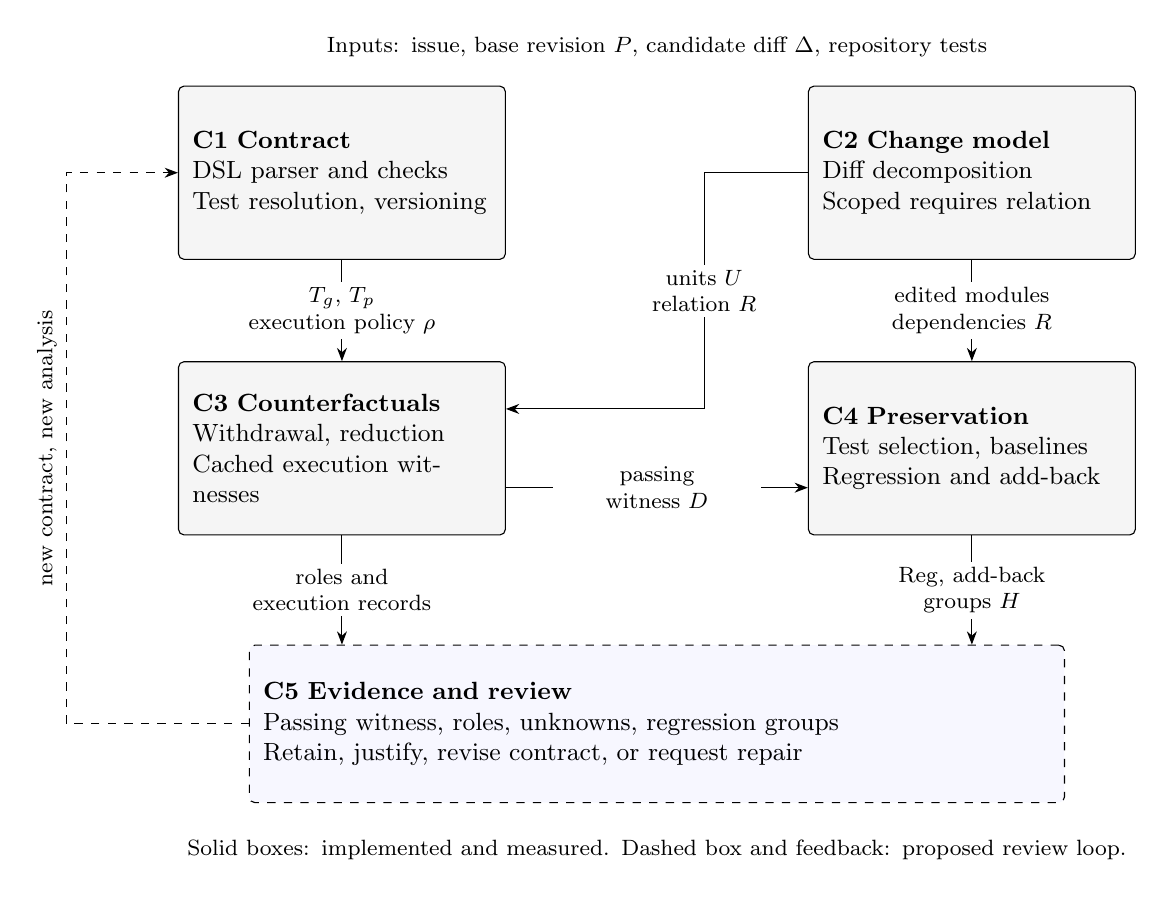
\begin{tikzpicture}[font=\small,>=Stealth,
 box/.style={draw,rounded corners=2pt,align=left,text width=38mm,minimum height=22mm,inner sep=5pt},
 proposed/.style={box,dashed,fill=blue!3},
 measured/.style={box,fill=black!4},
 lab/.style={font=\footnotesize,fill=white,inner sep=2pt,align=center}]
\node[measured] (c1) at (0,0) {\textbf{C1 Contract}\\DSL parser and checks\\Test resolution, versioning};
\node[measured] (c2) at (8,0) {\textbf{C2 Change model}\\Diff decomposition\\Scoped requires relation};
\node[measured] (c3) at (0,-3.5) {\textbf{C3 Counterfactuals}\\Withdrawal, reduction\\Cached execution witnesses};
\node[measured] (c4) at (8,-3.5) {\textbf{C4 Preservation}\\Test selection, baselines\\Regression and add-back};
\node[proposed,text width=100mm,minimum height=20mm] (c5) at (4,-7.0) {\textbf{C5 Evidence and review}\\Passing witness, roles, unknowns, regression groups\\Retain, justify, revise contract, or request repair};
\draw[->] (c1.south) -- node[lab,text width=38mm]{$T_g$, $T_p$\\execution policy $\rho$} (c3.north);
\draw[->] (c2.south) -- node[lab,text width=32mm]{edited modules\\dependencies $R$} (c4.north);
\draw[->] (c2.west) -- (4.6,0) -- node[lab,text width=19mm]{units $U$\\relation $R$} (4.6,-3.0) -- ([yshift=5mm]c3.east);
\draw[->] ([yshift=-5mm]c3.east) -- node[lab,text width=25mm]{passing\\witness $D$} ([yshift=-5mm]c4.west);
\draw[->] (c3.south) -- node[lab,text width=28mm]{roles and\\execution records} (c3.south |- c5.north);
\draw[->] (c4.south) -- node[lab,text width=28mm]{$\operatorname{Reg}$, add-back\\groups $H$} (c4.south |- c5.north);
\draw[->,dashed] (c5.west) -- (-3.5,-7.0) -- node[font=\footnotesize,rotate=90,above]{new contract, new analysis} (-3.5,0) -- (c1.west);
\node[font=\footnotesize,align=center,text width=120mm] at (4,1.6) {Inputs: issue, base revision $P$, candidate diff $\Delta$, repository tests};
\node[font=\footnotesize,align=center,text width=120mm] at (4,-8.6) {Solid boxes: implemented and measured. Dashed box and feedback: proposed review loop.};
\end{tikzpicture}
\caption{Architecture and evidence flow. C1 compiles a \dsl{} document into the executable inputs; the review loop is proposed. C4 also receives the contract's envelope policy $\eta$. In the retrospective study it inspects the reference patch to filter reference-observed test changes. A deployment would require explicit adjudication of such changes instead.}
\label{fig:architecture}
\end{figure}

\subsection{Overview}\label{sec:overview}

A patch that passes the available tests may still contain edits that do not contribute to the intended repair, while removing apparently unnecessary changes may break dependencies or introduce regressions. To address this problem, \tool{} assesses edit contributions through behavioral contracts and dependency-aware counterfactual execution, as illustrated in Figure~\ref{fig:architecture}. The approach consists of five components. First, C1 specifies the required repair behavior, preservation obligations, and execution policy (Section~\ref{sec:dsl}). C2 decomposes the patch into edit units and identifies dependencies to ensure that counterfactual variants preserve known structural requirements (Section~\ref{sec:decomposition}). C3 systematically evaluates edit withdrawals, identifies a reduced patch that satisfies the contract, and characterizes the contribution of each edit using execution evidence (Section~\ref{sec:triage}). Since passing the specified tests does not guarantee preservation of untested behavior, C4 selects additional tests and investigates potential regressions through add-back experiments (Section~\ref{sec:envelope}). Finally, C5 organizes the resulting evidence to support human review and subsequent agent revisions (Section~\ref{sec:review}). 


\subsection{C1: Behavioral contracts and executable outcomes}\label{sec:dsl}


To determine whether an edit contributes to a repair, we first specify what the patch must fix and which existing behavior it must preserve. We express these expectations in a behavioral contract, following the principle of making expected behavior explicit~\citep{meyer1992dbc}. The contract describes the required outcomes and leaves the choice of files and implementation strategy open. Executable tests provide evidence that a patch meets these requirements for the cases they exercise~\citep{barr2015oracle}.




\begin{definition}[Behavioral contract]\label{def:contract} For a base revision $P$, a \emph{behavioral contract} is a tuple $K=(T_g,T_p,\eta,\rho)$. The nonempty set $T_g$ contains tests that check whether a variant fixes the reported defect, and $T_p$ contains tests that check whether it preserves specified behavior of $P$. Together, $T_g\cup T_p$ defines the contract's \emph{core obligations}. The policy $\eta$ selects supplementary tests that probe additional preservation concerns. These tests form the \emph{preservation envelope}. The policy $\rho$ governs repeated test execution and determines when the available evidence is sufficient to assign a verdict. \end{definition}

The core obligations determine whether an edit can be removed under $K$. The preservation envelope probes what else might break after that removal. For example, a variant that omits an edit may pass every core test but fail a supplementary test that the full patch passes. The variant remains valid under $K$, and the supplementary failure identifies a potential regression that the core tests did not detect. Making that test a core obligation changes the contract and requires a fresh analysis.

For an edit configuration $S$ (defined in C2), the contract oracle $\mathcal{O}_K(S)$ evaluates the corresponding variant. It returns \lab{invalid} if the variant cannot be constructed or parsed. For a variant that can be evaluated, the oracle checks the goal tests first. It returns \lab{goal-fail} if a goal test fails. Once all goal tests pass, it returns \lab{pres-fail} if a core preservation test fails or \lab{valid} if all core obligations pass. If the available evidence is insufficient to determine a verdict under $\rho$, it returns \lab{unknown}. We write \begin{equation} \Valid_K(S)\quad\Longleftrightarrow\quad \mathcal{O}_K(S)=\lab{valid}. \label{eq:valid} \end{equation} The labels \lab{invalid} and \lab{unknown} record limits on evaluation. A \lab{valid} verdict establishes that the variant passes the core tests, with the conclusion limited to the behavior those tests exercise.



\paragraph{Contract notation.} \dsl{} is a textual form of the contract. It lets reviewers see which tests a patch must pass, which additional tests may be selected, and how the analysis gathers evidence. The notation leaves repair locations and implementation choices open. Its frontend parses a document, applies the static rules below, resolves test aliases, validates the base revision, and returns the contract $K$ that the analysis executes. Section~\ref{sec:contracts-eval} reports its application to every evaluated task. The interactive review authorization in C5 remains a proposed extension.

Listing~\ref{lst:dsl} shows the contract for the running example. The \code{goal} block names the test for the reported defect, and the \code{preserve} block names the set of 52 preservation tests described in Section~\ref{sec:running}. Both aliases resolve to exact test identifiers in a pinned catalog. The \code{envelope} declaration asks the implemented import-based policy to select up to six additional test modules. The first \code{evidence} declaration sets the number of full-patch executions for the stability check to two. The second specifies that the analysis tests edit withdrawals and searches for a reduced variant that passes the core tests. The optional \code{note} records the rationale for reviewers and has no effect on execution.

\begin{lstlisting}[numbers=left,caption={\dsl{} contract for the running example.},label=lst:dsl]
intent django_13297 {
  goal url_parameter {
    test catalog.template_params_filtering
  }
  preserve existing_views {
    tests catalog.generic_view_preservation
  }
  envelope import_rts top 6
  evidence full_repeats 2
  evidence counterfactual withdraw_and_reduce
  note "Wrapped URL values remain usable in queries"
}
\end{lstlisting}

Listing~\ref{lst:grammar} defines the core syntax. A contract has at least one goal block and may have zero or more preservation blocks. Block names are unique within a contract. A \code{test} reference resolves to one executable test, and a \code{tests} reference resolves to a finite set of tests. Identifiers begin with a letter and may also contain digits and underscores. Catalog references consist of dot-separated identifiers. Positive integers use decimal notation. Strings are double-quoted and support escaped quotes and backslashes.

\begin{lstlisting}[numbers=none,basicstyle=\ttfamily\small,caption={Core grammar of \dsl{}, as implemented in the frontend. Quoted tokens are terminals.},label=lst:grammar]
Contract ::= "intent" Id "{" Goal+ Preserve* Env
             Repeats Counterfactual Note? "}"
Goal     ::= "goal" Id "{" "test" TestRef "}"
Preserve ::= "preserve" Id "{" "tests" TestSetRef "}"
Env      ::= "envelope" "import_rts" "top" PositiveInt
Repeats  ::= "evidence" "full_repeats" PositiveInt
Counterfactual ::= "evidence" "counterfactual"
                   "withdraw_and_reduce"
Note     ::= "note" String
\end{lstlisting}


\paragraph{Static validation.} The compiler first resolves all test aliases against the pinned catalog. It rejects the contract if any alias is unresolved, if a block name appears more than once, or if a goal alias resolves to anything other than exactly one test. After resolution, each test identifier may appear in at most one of the two core sets, $T_g$ and $T_p$. The envelope size must be positive, and the stability check must request at least two full-patch executions.

\paragraph{Baseline validation.} Before evaluating the submitted patch, the analysis runs the core tests on the unpatched base revision $P$. The goal tests must reproduce the expected failures, and all core preservation tests must pass. If either expectation is unmet, the analysis stops and reports a baseline mismatch for diagnosis. It assigns no verdict to the submitted patch.

\paragraph{Execution semantics.} Compiling a \dsl{} specification produces the contract $K$ and binds it to a resolved test catalog, a base revision, and an execution environment identifier. The evidence policy $\rho$ governs repeated runs and determines when the available results support a verdict. If the evidence is insufficient, the oracle returns \lab{unknown}. The compiler returns a digest of these inputs. The analysis stores it with the submitted patch so that readers can identify the obligations and execution context under which a witness was obtained.

An agent may propose a contract amendment. If adopted, the amendment defines a new analysis, and earlier evidence remains bound to the original contract. For example, if an amendment removes a failing preservation test, a witness that passes under the amended contract establishes only that it meets the amended obligations. This distinction is especially important when the same agent proposes both the patch and the tests used to judge it. The current study evaluates patches against benchmark-defined obligations. Agent-authored contracts and amendments remain outside the scope of the evaluation.










Algorithm~\ref{alg:compile} describes how the \dsl{} frontend turns a textual specification into a contract that the analysis can execute. It first parses the specification and resolves test aliases against the pinned catalog. It then checks the resolved tests and policy settings against the static rules above. If those checks succeed, it runs the core tests on the unpatched base revision to verify that the goal tests reproduce the reported defect and that the preservation tests pass. Only after both checks succeed does the frontend return the contract and its execution context. A syntax error, a violated static rule, or a baseline mismatch produces a diagnostic before the submitted patch is evaluated. Every failure produces a diagnostic with a rule identifier and, for syntax errors, a source position. The frontend reports all static violations together instead of stopping at the first. Section~\ref{sec:future} outlines how to compare textual and structured input formats on authoring accuracy, comprehension, and maintenance while holding the analysis itself fixed.

\paragraph{Running example.} Applying Algorithm~\ref{alg:compile} to the Django contract in Listing~\ref{lst:dsl} proceeds as follows.

\begin{enumerate} \item \textbf{Parse the specification.} The frontend reads the contract name \code{django\_13297}, the two named test blocks, and the envelope and evidence declarations. The note records why wrapped URL values matter for the repair.

\item \textbf{Resolve the test aliases.} In the pinned catalog, the alias in \code{url\_parameter} resolves to one goal test for URL parameter filtering, which becomes $T_g$. The alias in \code{existing\_views} resolves to the 52 preservation tests, which become $T_p$.

\item \textbf{Check the static rules.} The frontend checks that the block names are distinct, that the goal alias resolves to exactly one test, and that its test identifier does not appear in $T_p$. The envelope limit of six satisfies the positive size requirement, and the two full-patch executions meet the minimum for the stability check.

\item \textbf{Validate the base revision.} The frontend runs the resolved core tests on the unpatched Django revision. The goal test must reproduce the reported failure, and all 52 preservation tests must pass. If either expectation is unmet, the frontend reports the baseline mismatch and stops before evaluating the patch.

\item \textbf{Return the validated contract.} If the baseline check succeeds, the frontend returns $K$ together with the resolved catalog, base revision, and environment identifier. The subsequent analysis uses the declared policies to check full-patch stability, test edit withdrawals, search for a reduced passing variant, and select up to six supplementary test modules for preservation checks. \end{enumerate}




\begin{algorithm}[H]
\caption{Contract compilation and preparation (C1)}\label{alg:compile}
\begin{algorithmic}[1]
\Require document $q$, catalog $A$, base $P$, environment $e$
\Ensure resolved contract and identity, or a diagnostic
\State $a\gets\Call{Parse}{q}$
\State \Call{CheckGrammarAndNames}{$a$}
\State $T_g\gets\Call{ResolveGoals}{a,A}$
\State $T_p\gets\Call{ResolvePreservation}{a,A}$
\State \Call{CheckCardinalityAndDisjointness}{$T_g,T_p$}
\State $\eta\gets\Call{ResolveEnvelope}{a}$
\State $\rho\gets\Call{ResolveEvidencePolicy}{a}$
\State \Call{CheckPolicyValues}{$\eta,\rho$}
\State $b\gets\Call{ExecuteBase}{P,T_g,T_p,e}$
\If{base expectations do not reproduce in $b$}
  \State \Return \Call{Diagnostic}{$b$}
\EndIf
\State \Return $(T_g,T_p,\eta,\rho),\Call{Digest}{P,e,A,a}$
\end{algorithmic}
\end{algorithm}




























% \subsection{C2: Dependency-aware change representation}\label{sec:decomposition}

% A file-level patch can contain several unrelated modifications. To evaluate them separately, let $\Delta$ be a candidate diff against the base revision $P$, decomposed into edit units $U=\{u_1,\ldots,u_n\}$. The implementation uses maximal consecutive runs of changed lines within diff hunks and represents each created or deleted file as one unit. Thus, an edit unit may contain several lines. Retaining a subset $S\subseteq U$ produces the candidate variant $P\oplus S$, provided its changes can be applied to the base.

% Not all edit units can be retained independently. For example, a branch using a newly imported class may require the edit introducing that import. We represent this constraint by $R\subseteq U\times U$, where $(a,b)\in R$ means that retaining $a$ requires retaining $b$. The closure $\cl_R(S)$ repeatedly adds all required units. A configuration is \emph{closed} when $\cl_R(S)=S$.

% Removing a required unit must also remove any units that depend on it. Let $\operatorname{dep}_R(u)$ denote the units that transitively require $u$. The permitted withdrawal from a configuration $S$ is
% \begin{equation}
% \withdraw_R(S,u)=S\setminus\bigl(\{u\}\cup\operatorname{dep}_R(u)\bigr).
% \label{eq:withdraw}
% \end{equation}
% If $S$ is closed and contains $u$, the withdrawal yields a strictly smaller closed configuration. Accordingly, its outcome concerns an admissible group of edits rather than necessarily isolating the effect of one changed line. Closure is extensive, monotone, and idempotent for fixed $R$, but these properties do not establish that $R$ includes every runtime dependency.

% \paragraph{Construction and dependency extraction.}
% C2 locates each diff hunk against the unchanged base and reconstructs variants from that revision. Protected benchmark test files are excluded because the evaluation harness installs its own test patch. Other test and auxiliary edits remain in the change model, but their removability is interpreted separately from source-code behavior.

% The implemented requires relation uses newly introduced or removed bindings. When an added use refers to a name that another unit newly binds, C2 records a requires edge. Conversely, when a unit removes a binding whose remaining uses another unit removes, the two are linked. Imports and assignments are matched within their module, because Python binds them per module. New functions and classes can establish cross-file edges through name-based matching. This relation is an approximation for Python. Dynamic imports, aliases, monkey patching, reflection, and implicit framework behavior may escape it. Conversely, name matching can add a spurious edge and force units to remain together. All guarantees are relative to the resulting admissible configurations.

% Every constructed Python variant undergoes a parse check before test execution. A parse rejection avoids an expensive run, but it is not evidence that the withdrawn edit is behaviorally essential. Closed configurations can still fail at runtime because the dependency model is incomplete. The report records whether a rejection came from the precheck or from execution, so that these differences are not hidden behind a single semantic necessity claim.

% \paragraph{Running example.}
% The adapter branch $u_2$ uses the name that $u_1$ introduces, and the field branch $u_4$ uses the name that $u_3$ adds to an existing import. Thus
% \[
% R=\{(u_2,u_1),(u_4,u_3)\}.
% \]
% Although both providers import \code{LazyObject}, they bind it in different modules. Linking either branch to the other module's import would create a false dependency. An earlier implementation matched imports across files and made the unneeded import $u_1$ appear necessary. This case led to the per-module scoping rule, and all affected records were rerun. Withdrawing $u_3$ now removes $u_4$, while $u_1,u_2$ remain available. The recorded ablation without closure shows why the relation matters. It executed $\{u_4\}$ alone, which parses but references a name that is not bound. That run failed the goal test and all 52 preservation tests, an outcome caused by a broken variant rather than by behavioral necessity.

% \subsection{C3: Counterfactual execution and edit roles}\label{sec:triage}

% C3 asks two complementary questions. What happens when a unit and its dependents are withdrawn from the full patch? And can a smaller, dependency-closed subset of the patch still satisfy the contract? The first question provides evidence about each full-patch withdrawal. The second identifies a \emph{passing witness} $D\subseteq U$, whose omitted units can be removed together under the observed obligations. Neither observation alone establishes that an edit is present in every possible valid repair.

% The analysis first checks that the base reproduces the failure and that the full patch passes repeatedly. Repeated runs bypass the outcome cache. Patches that do not reproduce these preconditions are reported as unresolved. Full-patch stability does not establish that all subsets behave deterministically, so unknown outcomes are never treated as passing reductions. Section~\ref{sec:rq4} evaluates agreement across repeated configurations.

% C3 tests the permitted withdrawal $\withdraw_R(U,u)$ for each $u\in U$. It then applies \textsc{ddmin}~\citep{zeller2002ddmin} to find a smaller passing configuration, closing candidates under $R$ before execution. Because closure may reintroduce required units, \textsc{ddmin}'s ordinary 1-minimality result does not automatically transfer to the closed witness. A final pass therefore repeatedly accepts any passing withdrawal from the current closed witness. Algorithm~\ref{alg:triage} specifies this procedure.

% \paragraph{Contextual edit roles.}
% A passing full patch can contain alternative or compensating repairs. We therefore characterize an edit using both its membership in $D$ and its full-patch withdrawal result $o_u=\mathcal{O}_K(\withdraw_R(U,u))$.

% \begin{definition}[Operational edit roles]\label{def:roles}
% For a valid full patch $U$ and a valid witness $D$, each unit with a conclusive full-patch withdrawal outcome has one of four contextual roles:
% \begin{center}
% \begin{tabular}{lll}
% \toprule
% Role & Membership in $D$ & Full-patch withdrawal \\
% \midrule
% \lab{N}: retained, withdrawal-sensitive & $u\in D$ & rejected \\
% \lab{J}: retained alternative & $u\in D$ & valid \\
% \lab{C}: omitted, withdrawal-sensitive & $u\notin D$ & rejected \\
% \lab{U}: omitted, individually removable & $u\notin D$ & valid \\
% \bottomrule
% \end{tabular}
% \end{center}
% A rejected withdrawal has a completed non-valid outcome, including structural rejection. A unit whose withdrawal outcome is unknown receives \lab{X}. Units labeled \lab{C} or \lab{U} are \emph{removable} because they are absent from the same passing witness, even when removing them individually from the full patch fails.
% \end{definition}

% These labels describe observations in particular configurations, not global properties of the edits. In particular, \lab{N} does not imply that the unit appears in every valid repair. \lab{J} identifies a retained edit that can be withdrawn from the full patch, while \lab{C} identifies an edit omitted by a passing witness despite a rejected full-patch withdrawal. The implementation calls these roles \emph{necessary}, \emph{jointly needed}, \emph{coupled}, and \emph{unneeded}, respectively. We retain the symbols used in the results but interpret them operationally.

% \begin{algorithm}[tbp]
% \caption{Dependency-aware counterfactual triage (C3)}\label{alg:triage}
% \begin{algorithmic}[1]
% \Require units $U$, relation $R$, contract oracle $\mathcal{O}_K$
% \Ensure passing witness, contextual roles, and execution evidence
% \State $b\gets\Call{CheckBaseAndRepeatedFull}{U,K}$
% \If{$b$ does not establish the preconditions}
%   \State \Return \Call{UnresolvedReport}{$b$}
% \EndIf
% \For{each $u\in U$}
%   \State $o_u\gets\mathcal{O}_K(\withdraw_R(U,u))$
% \EndFor
% \State $D\gets\cl_R(\Call{DDMin}{U,\Valid_K\circ\cl_R})$
% \State $W\gets\Call{FindPassingWithdrawal}{D,R,K}$
% \While{$W\ne\lab{none}$}
%   \State $D\gets W$
%   \State $W\gets\Call{FindPassingWithdrawal}{D,R,K}$
% \EndWhile
% \State $L\gets\Call{AssignOperationalRoles}{D,\{o_u\}_{u\in U}}$
% \State \Return $D,L,\Call{ExecutionEvidence}{K}$
% \end{algorithmic}
% \end{algorithm}

% \textsc{AssignOperationalRoles} applies Definition~\ref{def:roles} to $D$ and $o_u$. Under standard bounds for the chosen \textsc{ddmin} implementation and assuming individual oracle invocations terminate, the procedure uses $n+O(n^2)$ oracle queries in the worst case. The withdrawals contribute $n$, \textsc{ddmin} contributes $O(n^2)$, and the final pass contributes at most $n$ withdrawals per accepted reduction. In practice, caching and small patches keep the count low (Section~\ref{sec:rq4}). The cache avoids rerunning an identical configuration within a session, but it does not turn a nondeterministic test into a deterministic one. Cached outcomes are valid only for the same base, patch, contract, and environment. Cross-session cache reuse would require checking these identities and specifying a stability policy.

% \begin{proposition}[Passing witness and withdrawal minimality]\label{prop:minimality}
% Assume a deterministic oracle, a closed valid full patch, and completed non-unknown outcomes for the final withdrawal neighborhood. Algorithm~\ref{alg:triage} returns a closed valid witness $D$ such that, for every $u\in D$, $\withdraw_R(D,u)$ is not valid.
% \end{proposition}
% \begin{proof}
% The initial full patch is valid. Closure-aware \textsc{ddmin} and every accepted withdrawal preserve an observed valid closed configuration. Equation~\ref{eq:withdraw} removes a retained unit and all its dependents, so it yields a closed strict subset. Each accepted withdrawal therefore decreases the finite set $D$, and the loop terminates. At termination every permitted withdrawal has been considered and none is valid. Determinism and completed outcomes give the stated property.
% \end{proof}

% If a final withdrawal times out, the observed property is weaker: no tested withdrawal was accepted, but at least one possibility remains unknown. Such a run does not establish behavioral irreducibility. The records retain \lab{X} for unknown full-patch withdrawals, but they lack a separate certification flag for every uncertainty in the final neighborhood. We therefore report observed witness reductions rather than a certified guarantee for every empirical patch.

% \begin{proposition}[Omission witness]\label{prop:omission}
% For every unit $u\notin D$, the returned $D$ is a passing configuration that omits $u$. The complete omitted set $U\setminus D$ can therefore be removed together while preserving the observed core obligations.
% \end{proposition}
% \begin{proof}
% The algorithm accepts a reduced configuration only after a valid outcome. Membership in $U\setminus D$ means that the corresponding unit is absent from that passing witness.
% \end{proof}

% These results are useful without implying global necessity or correctness. An \lab{N} withdrawal fails from the full patch, yet another repair subset might still omit that unit. An omitted edit can remain useful under an untested requirement. The output is an evidence-bearing review aid, not proof that the omitted changes are poor engineering.

% \paragraph{Running example.}
% Table~\ref{tab:example} lists the decisive configurations. The withdrawal outcomes and the passing witness yield \lab{U} for $u_1,u_2$ and \lab{N} for $u_3,u_4$. The run used eight oracle executions in total. Two were full-patch checks and one was the base check, four were withdrawals, and \textsc{ddmin} added one new configuration, $\{u_3\}$. The closure of $\{u_4\}$ is the cached witness, so that generator required no new run. The classification does not depend on proximity to the maintainer's view repair.

% \begin{table}[pos=htbp]
% \caption{Decisive running-example configurations (recorded). Every valid row also satisfies the 52 preservation obligations. The repeated full-patch run and the \textsc{ddmin} probe $\{u_3\}$ (goal-fail) are not shown.}
% \label{tab:example}
% \centering\small
% \begin{tabular}{lll}
% \toprule
% Purpose & Retained units & Core outcome \\
% \midrule
% Base & $\emptyset$ & goal-fail \\
% Full candidate & $u_1,u_2,u_3,u_4$ & valid \\
% Withdraw $u_1$ and dependent $u_2$ & $u_3,u_4$ & valid \\
% Withdraw $u_2$ & $u_1,u_3,u_4$ & valid \\
% Withdraw $u_3$ and dependent $u_4$ & $u_1,u_2$ & goal-fail \\
% Withdraw $u_4$ & $u_1,u_2,u_3$ & goal-fail \\
% Witness $D$ & $u_3,u_4$ & valid \\
% \bottomrule
% \end{tabular}
% \end{table}

% The case has no retained alternative and no omitted withdrawal-sensitive unit. Two synthetic cases illustrate those roles without inventing repository results. If either of two edits independently repairs a defect, the retained one receives \lab{J}, because withdrawing it from the full patch leaves the other repair in place. If two compensating edits can be omitted together but not separately, the omitted units receive \lab{C}. These possibilities show that one-at-a-time deletion alone does not fully describe edit contribution. Section~\ref{sec:rq4} reports recorded instances of both roles.

% \subsection{C4: Preservation beyond the core obligations}\label{sec:envelope}

% Passing $T_g\cup T_p$ leaves behavior outside those tests unobserved. C4 therefore selects additional test modules using the candidate's actual edited source modules. The implemented import-based score combines direct imports, matching test filenames, package affinity, and proximity to the original test directories. It retains up to $k$ modules above a minimum score. This is a heuristic selection policy, not safe regression test selection, so its recall must be measured.

% C4 runs the selected tests twice on the base and retains tests observed to pass both times. In the retrospective experiment it also runs the reference patch and excludes tests that fail there. This exclusion avoids automatically calling every reference-observed behavior change a regression, but it does not prove that the excluded behavior is intended. We therefore call the output a \emph{reference-filtered preservation signal}. A deployment without a reference patch would instead adjudicate the affected tests against the contract. An unavailable test result must remain unknown rather than count as a confirmed regression.

% Let $T_E$ be the selected tests, $B$ the tests passing in both base runs, and $F(S)$ the completed failures on configuration $S$. Let $A$ contain tests excluded by the retrospective reference check or by explicit contract adjudication. The observed regression set is
% \begin{equation}
% \operatorname{Reg}(S)=\bigl(B\cap F(S)\bigr)\setminus(A\cup T_g).
% \label{eq:regression}
% \end{equation}
% The implementation approximates this set by passing-set differences, which can also include unreported or interrupted tests. Every recorded regression was therefore re-executed in a fresh container, and only reproducing regressions are reported. The result remains subject to the harness's ability to distinguish failure from missing evidence.

% If a regression disappears in $D$, C4 adds omitted units back to investigate it. An add-back can also include required support edits. Its observation implicates that closed group relative to $D$. It does not prove that one edit alone causes the failure in every context. Regressions already present in $D$ reveal a limitation of the core obligations that reduction cannot remove.

% \begin{algorithm}[tbp]
% \caption{Envelope observations and add-back witnesses (C4)}\label{alg:envelope}
% \begin{algorithmic}[1]
% \Require base $P$, full units $U$, relation $R$, witness $D$, policy $\eta$, exclusions $A$
% \Ensure regression observations and implicated groups
% \State $T_E\gets\Call{SelectAdditionalTests}{P,U,\eta}$
% \State $B\gets\Call{StablePassingTests}{P,T_E}$
% \State $G\gets\operatorname{Reg}(U)$ \Comment{Equation~\ref{eq:regression} on $T_E$}
% \State \textbf{if} $G=\emptyset$ \textbf{then return} $\emptyset,\emptyset,\emptyset$
% \State $G_D\gets\operatorname{Reg}(D)\cap G$
% \State $H\gets\emptyset$
% \For{each $u\in U\setminus D$}
%   \State $S\gets\cl_R(D\cup\{u\})$
%   \State $g\gets(G\setminus G_D)\cap\operatorname{Reg}(S)$
%   \If{$g\ne\emptyset$} \State $H\gets H\cup\{(S\setminus D,g)\}$ \EndIf
% \EndFor
% \State \Return $G,G_D,H$
% \end{algorithmic}
% \end{algorithm}

% Algorithm~\ref{alg:envelope} formalizes the intended evidence semantics, rather than an exact representation of every implementation detail. It requires two base runs, one full and one witness run when a regression occurs, and one add-back run per omitted unit. The existing add-back implementation adds the unit and its direct requirements rather than the full transitive closure, which differs only when requirement chains are longer than one edge. The \lab{H} tag in the records should therefore be read as an add-back association under that implementation, not as proof of isolated causal responsibility. Failures that arise only from interactions among several omitted groups can also escape individual add-backs.

% \paragraph{Running example.}
% C4 selects tests using the two database modules that the agent edited, even though the contract's original tests concern generic views. The selected modules include the base backend operation tests. The envelope contains 75 tests observed to pass on the base, and no envelope regression is recorded for the full candidate. Now suppose that a separately completed envelope test failed only after adding the omitted adapter route back to $D$. The report would then attach that test and the added group as a preservation witness. This hypothetical continuation explains the mechanism without converting an unobserved result into evidence.

% \subsection{C5: Evidence for review and agent feedback}\label{sec:review}

% The proposed report joins the resolved contract, unit definitions, requires edges, passing witness, withdrawal outcomes, and preservation observations. For each unit, it states whether the unit is retained, whether its full-patch withdrawal passes, and whether missing evidence limits the classification. It also records which additional tests were selected and which failures a reference-based rule excluded. An omission recommendation without these details would hide the conditions on which it depends.

% The intended workflow offers three actions. A maintainer can review the passing witness first, retain an omitted edit with an explicit additional requirement, or request a repair when preservation fails. Adding a justified requirement changes the contract and triggers a new analysis. An agent can receive the same evidence and revise its patch, but its explanation does not replace the witness. The report does not delete logging, comments, defensive changes, or other edits merely because the current test suite does not require them.

% \paragraph{Running example.}
% The report would show $\{u_3,u_4\}$ as the passing core and $\{u_1,u_2\}$ as an omitted adapter route. A reviewer can ask whether adapter support is a separately desired requirement. If it is, that requirement needs its own executable evidence or explicit manual justification. The reduced patch still needs review for private-attribute access and untested lazy-evaluation behavior. In this way a higher-level contract governs different repair routes without equating minimality with engineering quality.
















% %=========





\subsection{C2: Dependency-aware change representation}\label{sec:decomposition}

A patch can implement several changes in the same file, and a single change can depend on edits elsewhere in the patch. C2 divides the submitted diff $\Delta$ into units that can be tested in combination and records which units must be retained together. C3 uses this representation to build the variants it evaluates.

\paragraph{Edit units and variant construction.} Let $P$ be the base revision and $U=\{u_1,\ldots,u_n\}$ the units extracted from $\Delta$. Within each diff hunk, a maximal consecutive run of changed lines forms one unit. A newly created or deleted file forms one unit. An \emph{edit configuration} $S\subseteq U$ specifies which units to retain. To construct the variant $P\oplus S$, C2 locates the original hunks against $P$ and applies the selected changes from that base. In the benchmark study, the harness installs its own protected test patch, and edits to those protected files are excluded from $U$. Other test and auxiliary edits remain in the representation, and their roles are reported separately from those of source edits.

\paragraph{Requires relation.} Retaining a branch that refers to a newly imported name may also require retaining the import. We write $(a,b)\in R$ when retaining edit $a$ requires retaining edit $b$. The closure $\cl_R(S)$ adds the required units and follows their requirements until no further unit must be added. A configuration $S$ is \emph{closed} if $\cl_R(S)=S$. Closure is extensive, monotone, and idempotent for a fixed $R$. Its coverage depends on which requires edges C2 detects.

\paragraph{Dependency-aware withdrawal.} Removing a required edit also removes every retained edit that requires it, directly or through a chain of edges. Let $\operatorname{dep}_R(u)$ denote all units that transitively require $u$. The permitted withdrawal of $u$ from $S$ is
\begin{equation}
\withdraw_R(S,u)=S\setminus\bigl(\{u\}\cup\operatorname{dep}_R(u)\bigr).
\label{eq:withdraw}
\end{equation}
If $S$ is closed and contains $u$, the withdrawal yields a strictly smaller closed configuration. A withdrawal verdict therefore applies to the whole group removed by Equation~\ref{eq:withdraw}.

\paragraph{Dependency extraction and structural checks.} C2 adds an edge from a unit that introduces a use of a name to the unit that introduces its binding. For deletions, a unit that removes a binding requires units that remove uses that would otherwise remain. C2 matches imports and assignments within their module. It can also match newly introduced function and class names across files. These rules approximate Python dependencies. Dynamic imports, aliases, monkey patching, reflection, and framework behavior can hide dependencies, and name matching can introduce false edges. C2 checks that each constructed Python variant parses before passing it to the oracle. A parse rejection records a structural problem. A closed variant that parses can still fail at runtime if a dependency was missed.

\paragraph{Running example.} C2 constructs the representation for the Django patch in Listing~\ref{lst:running} in three steps.
\begin{enumerate}
\item \textbf{Identify the units.} The backend adapter contributes the import $u_1$ and the branch $u_2$ that uses it. Model field preparation contributes the import change $u_3$ and the branch $u_4$ that uses it.
\item \textbf{Link each use to its binding.} The adapter branch uses the binding introduced by $u_1$, and the field branch uses the binding introduced by $u_3$. Thus $R=\{(u_2,u_1),(u_4,u_3)\}$. Both modules bind \code{LazyObject} locally. An earlier cross-file import match incorrectly made $u_1$ appear necessary. The implementation was corrected to scope import matches by module, and the affected cases were rerun.
\item \textbf{Construct an admissible variant.} Withdrawing $u_3$ from the full patch also removes $u_4$, leaving $\{u_1,u_2\}$. Conversely, closing a configuration that contains only $u_4$ adds $u_3$. In the recorded ablation without closure, $\{u_4\}$ parsed but used an unbound name. The goal test and all 52 preservation tests failed. That run exposes the missing import in the constructed variant.
\end{enumerate}

\subsection{C3: Counterfactual execution and edit roles}\label{sec:triage}

C3 tests what happens when a unit and its dependents are withdrawn from the full patch. It also searches for a smaller closed configuration that still passes the core obligations. We call such a returned configuration a \emph{passing witness} $D\subseteq U$. The withdrawal verdict describes the effect of a specific removal from $U$, while $D$ shows which units can be omitted together under the contract.

\paragraph{Preconditions and search.} Algorithm~\ref{alg:triage} first checks that the full patch passes the core obligations on repeated runs and that the base revision does not. In all 1,674 evaluated records the base fails a goal test. The triage itself does not require the base to pass every core preservation test. That stronger check belongs to the contract frontend (Algorithm~\ref{alg:compile}), whose results are reported in Section~\ref{sec:contracts-eval}. Repeated runs bypass the outcome cache. The algorithm reports the patch as unresolved if these preconditions cannot be established. It then records the verdict of $\withdraw_R(U,u)$ for every $u\in U$ and runs \textsc{ddmin}~\citep{zeller2002ddmin} to find a smaller passing configuration. Every candidate is closed under $R$ before execution. Closure can reintroduce a unit that \textsc{ddmin} proposed removing, so the algorithm finishes by explicitly testing permitted withdrawals from the current closed witness. After each passing withdrawal, it restarts the check from the smaller witness. Only a \lab{valid} verdict can justify accepting a reduction.

\paragraph{Contextual edit roles.} To read a role, ask whether the final witness retains the unit and what happens when that unit and its dependents are withdrawn from the full patch. These observations can differ because the full patch may contain alternative repairs or edits whose effects depend on one another.

\begin{definition}[Operational edit roles]\label{def:roles}
For a valid full patch $U$ and a valid witness $D$, let $o_u=\mathcal{O}_K(\withdraw_R(U,u))$. The following table defines the role of $u$ when $o_u$ is conclusive.
\begin{center}
\begin{tabular}{lll}
\toprule
Role & Membership in $D$ & Full-patch withdrawal \\
\midrule
\lab{N}: retained, withdrawal-sensitive & $u\in D$ & rejected \\
\lab{J}: retained alternative & $u\in D$ & valid \\
\lab{C}: omitted, withdrawal-sensitive & $u\notin D$ & rejected \\
\lab{U}: omitted, individually removable & $u\notin D$ & valid \\
\bottomrule
\end{tabular}
\end{center}
A rejected withdrawal has a conclusive non-valid verdict, which may be a structural rejection or a test failure. A unit with an unknown full-patch withdrawal receives \lab{X}. The conclusive removable roles are \lab{C} and \lab{U}, since the passing witness omits both kinds of units.
\end{definition}

The implementation names \lab{N}, \lab{J}, \lab{C}, and \lab{U} \emph{necessary}, \emph{jointly needed}, \emph{coupled}, and \emph{unneeded}, respectively. In the results, each label refers to the tested configurations. For instance, \lab{N} means that the witness retains the unit and the specified withdrawal from the full patch was rejected. A different passing configuration could still omit it. Similarly, \lab{U} identifies a successful unit-initiated withdrawal, which may have removed dependents as well.

\begin{algorithm}[tbp]
\caption{Dependency-aware counterfactual triage (C3)}\label{alg:triage}
\begin{algorithmic}[1]
\Require units $U$, relation $R$, contract oracle $\mathcal{O}_K$
\Ensure passing witness, contextual roles, and execution evidence, or unresolved report
\State $b\gets\Call{CheckBaseAndRepeatedFull}{U,K}$
\If{$b$ does not establish the preconditions}
  \State \Return \Call{UnresolvedReport}{$b$}
\EndIf
\For{each $u\in U$}
  \State $o_u\gets\mathcal{O}_K(\withdraw_R(U,u))$
\EndFor
\State $D\gets\cl_R(\Call{DDMin}{U,\Valid_K\circ\cl_R})$
\State $W\gets\Call{FindPassingWithdrawal}{D,R,K}$
\While{$W\ne\lab{none}$}
  \State $D\gets W$
  \State $W\gets\Call{FindPassingWithdrawal}{D,R,K}$
\EndWhile
\State $L\gets\Call{AssignOperationalRoles}{D,\{o_u\}_{u\in U}}$
\State \Return $D,L,\Call{ExecutionEvidence}{K}$
\end{algorithmic}
\end{algorithm}

\paragraph{Execution cost and caching.} With $n$ units, the full-patch withdrawals issue $n$ oracle queries, \textsc{ddmin} issues $O(n^2)$ in the worst case, and the final pass issues at most $n$ queries per round over at most $n+1$ rounds. These bounds assume that individual oracle calls terminate. Within a session, the cache can reuse an outcome for the same configuration under the same base, patch, contract, and environment. Repeated executions remain necessary when measuring stability. Section~\ref{sec:rq4} reports execution counts and agreement across repeated configurations.

\begin{proposition}[Passing witness and withdrawal minimality]\label{prop:minimality}
Assume a deterministic oracle, a closed valid full patch, and a conclusive outcome for every permitted withdrawal from the final witness. Algorithm~\ref{alg:triage} returns a closed valid witness $D$ such that $\withdraw_R(D,u)$ is non-valid for every $u\in D$.
\end{proposition}
\begin{proof}
The search starts from the closed valid full patch. Closure-aware \textsc{ddmin} and the final withdrawal pass accept a configuration only after a valid verdict, so the current witness remains closed and valid. Every accepted withdrawal removes at least its selected unit, so the final pass terminates. The last round considers every permitted withdrawal from the returned $D$. None passes, and determinism and conclusive outcomes give the stated property.
\end{proof}

The proposition concerns the final witness's withdrawal neighborhood. If a final withdrawal times out, the passing witness still establishes the joint omission, but the timed-out withdrawal remains unresolved. The records use \lab{X} for unknown full-patch withdrawals and lack a separate certification flag for uncertainty in the final neighborhood. The empirical results therefore report observed witness reductions.

\begin{proposition}[Omission witness]\label{prop:omission}
The returned $D$ is a passing configuration that omits every unit in $U\setminus D$ simultaneously.
\end{proposition}
\begin{proof}
The returned configuration has a valid core verdict and contains exactly the units in $D$. Its verdict is therefore evidence that the entire omitted set can be removed together under the observed core obligations.
\end{proof}

\paragraph{Running example.} The recorded Django run follows Algorithm~\ref{alg:triage} as follows.
\begin{enumerate}
\item \textbf{Check the base and full patch.} The goal test fails on the base as expected. The full patch passes the goal test and all 52 preservation tests on both runs.
\item \textbf{Test full-patch withdrawals.} Table~\ref{tab:example} shows all four withdrawals. Removing the adapter import also removes the adapter branch, leaving the field route and a valid verdict. Removing just the adapter branch also passes. Removing either the field import and its dependent branch, or just the field branch, leaves a variant that fails the goal test.
\item \textbf{Find and check the witness.} The reduced witness is $D=\{u_3,u_4\}$. The search executes $\{u_3\}$ and observes a goal failure. Closing $\{u_4\}$ gives $\{u_3,u_4\}$, whose passing verdict is already cached. The final withdrawals from $D$ leave $\emptyset$ or $\{u_3\}$, both of which have recorded goal failures. The run uses eight oracle executions in total: one base check, two full-patch checks, four full-patch withdrawals, and one new reduction probe.
\item \textbf{Assign roles.} The witness omits $u_1$ and $u_2$, and both full-patch withdrawals pass, so these units receive \lab{U}. It retains $u_3$ and $u_4$, whose full-patch withdrawals fail the goal test, so these units receive \lab{N}.
\end{enumerate}

\begin{table}[pos=htbp]
\caption{Recorded core outcomes for the decisive Django configurations. Every valid configuration passes the goal test and all 52 preservation tests.}
\label{tab:example}
\centering\small
\begin{tabular}{lll}
\toprule
Purpose & Retained units & Core outcome \\
\midrule
Base & $\emptyset$ & goal-fail \\
Full candidate (two runs) & $u_1,u_2,u_3,u_4$ & valid \\
Withdraw $u_1$ and dependent $u_2$ & $u_3,u_4$ & valid \\
Withdraw $u_2$ & $u_1,u_3,u_4$ & valid \\
Withdraw $u_3$ and dependent $u_4$ & $u_1,u_2$ & goal-fail \\
Withdraw $u_4$ & $u_1,u_2,u_3$ & goal-fail \\
Reduction probe & $u_3$ & goal-fail \\
Witness $D$ & $u_3,u_4$ & valid \\
\bottomrule
\end{tabular}
\end{table}

Two hypothetical cases clarify the remaining roles. If either of two repair edits can fix the defect independently, the edit retained in a one-edit witness receives \lab{J}: its full-patch withdrawal leaves the other repair in place. If two compensating edits can be removed together but either individual withdrawal breaks a core test, both omitted units receive \lab{C}. Section~\ref{sec:rq4} reports recorded instances of both roles.

\subsection{C4: Preservation beyond the core obligations}\label{sec:envelope}

A passing core witness establishes that the contract's core tests pass. C4 uses the supplementary tests selected by $\eta$ to ask whether the full patch disrupts behavior those tests exercise and, if so, whether the same failure persists in the witness.

\paragraph{Select and qualify supplementary tests.} C4 ranks test modules against the candidate's edited source modules using imports, matching filenames, package affinity, and proximity to the original test directories. It selects up to $k$ modules above the minimum score. This heuristic can miss relevant tests. C4 runs the selected tests twice on the base and retains those observed to pass in both runs. In the retrospective study, C4 also runs the reference patch and excludes tests that fail there. The resulting \emph{reference-filtered preservation signal} records failures after that exclusion. The reference outcome alone cannot establish whether a behavior change was intended. In a deployment without a reference patch, a reviewer would adjudicate proposed exclusions against the contract.

\paragraph{Define the observed regressions.} Let $T_E$ be the selected tests, let $B\subseteq T_E$ contain the tests that pass in both base runs, and let $F(S)\subseteq T_E$ contain the completed failures on configuration $S$. Let $A$ contain tests excluded by the retrospective reference check or by explicit adjudication. The observed regression set is
\begin{equation}
\operatorname{Reg}(S)=\bigl(B\cap F(S)\bigr)\setminus(A\cup T_g).
\label{eq:regression}
\end{equation}
An observed regression thus requires both a stable pass on the base and a completed failure on the variant. The implementation approximates $F(S)$ by differences between passing sets, which can also capture unreported or interrupted tests. Every recorded regression was re-executed in a fresh container, and only reproducing regressions are reported. Interpretation still depends on the harness's ability to distinguish completed failures from missing results.

\paragraph{Compare the full patch and the witness.} Algorithm~\ref{alg:envelope} first identifies the regression set $G$ for the full patch. If $G$ is empty, there is no observed full-patch failure to trace. Otherwise, C4 runs the envelope on $D$ and records which failures persist in $G_D$. A completed pass on $D$ identifies a full-patch failure that disappears in the witness. For such a test, C4 investigates whether the failure reappears after adding an omitted unit and its required support edits to $D$. Each resulting association concerns the added group in the context of $D$. Interactions that require several omitted groups to be added together can escape this check.

\begin{algorithm}[tbp]
\caption{Envelope observations and add-back witnesses (C4)}\label{alg:envelope}
\begin{algorithmic}[1]
\Require base $P$, full units $U$, relation $R$, witness $D$, policy $\eta$, exclusions $A$
\Ensure full-patch regressions, persistent regressions, and add-back associations
\State $T_E\gets\Call{SelectAdditionalTests}{P,U,\eta}$
\State $B\gets\Call{StablePassingTests}{P,T_E}$
\State $G\gets\operatorname{Reg}(U)$ \Comment{Equation~\ref{eq:regression}}
\If{$G=\emptyset$} \State \Return $\emptyset,\emptyset,\emptyset$ \EndIf
\State $G_D\gets G\cap\operatorname{Reg}(D)$
\State $Q\gets G\cap\Call{CompletedPasses}{D,T_E}$
\State $H\gets\emptyset$
\For{each $u\in U\setminus D$ with $Q\ne\emptyset$}
  \State $S\gets\cl_R(D\cup\{u\})$
  \State $g\gets Q\cap\operatorname{Reg}(S)$
  \If{$g\ne\emptyset$} \State $H\gets H\cup\{(S\setminus D,g)\}$ \EndIf
\EndFor
\State \Return $G,G_D,H$
\end{algorithmic}
\end{algorithm}

The algorithm specifies the intended evidence semantics. The witness execution supplies both its completed passes and its completed failures. A test with an unavailable witness outcome supplies neither, so it cannot support an add-back claim. Beyond any reference run used to determine $A$, the procedure uses two base runs, one full-patch run, one witness run if a full-patch regression is observed, and at most one add-back run per omitted unit. The campaign's implementation added only direct requirements, whereas the pseudocode closes the configuration transitively. We have since aligned the implementation with the pseudocode. In all 25 records with an envelope regression the two configurations coincide for every omitted unit, so the recorded \lab{H} associations are unaffected.

\paragraph{Running example.} C4 applies the envelope policy to the same Django patch in three steps.
\begin{enumerate}
\item \textbf{Select tests from the edited modules.} The edited backend operations and model field modules guide selection. The selected modules include the base backend operation tests, extending the coverage provided by the generic-view preservation obligations.
\item \textbf{Compare with the base.} The envelope contains 75 tests observed to pass on the base. The full candidate has no recorded envelope regression, so there is no observed failure to compare against the reduced witness or trace through add-backs.
\item \textbf{Illustrate the add-back branch.} Suppose an envelope test had passed on the base and on $D=\{u_3,u_4\}$, failed on the full patch, and remained eligible after reference filtering. Adding the omitted adapter branch $u_2$ to $D$ would also add its required import $u_1$. If the test then failed again, C4 would record an association with the group $\{u_1,u_2\}$ in the context of $D$. This is a hypothetical execution of the add-back branch.
\end{enumerate}

\subsection{C5: Evidence for review and agent feedback}\label{sec:review}

C5 proposes a report that lets a reviewer inspect the evidence behind a reduced patch. It brings together the resolved contract, edit units and their dependencies, the passing witness, and the full-patch and withdrawal verdicts. Each unit entry identifies whether the witness retains it, which other units its withdrawal removes, and whether the outcome is conclusive. The preservation section lists the supplementary tests that were selected, failures excluded by the reference filter, and any observed regressions or add-back associations. The interactive review and agent-feedback workflow is proposed. The evaluation measures the executable evidence produced by C2--C4.

\paragraph{Review decisions.} A maintainer can inspect the passing witness as a candidate for review, retain an omitted edit for a separately justified requirement, or request a revision when a preservation failure needs attention. Adding a requirement to the core obligations creates a revised contract and calls for a fresh analysis. A maintainer can also document a manual engineering reason to retain an edit, such as a logging or defensive change. If an agent revises the patch, its explanation can guide the review, and a new execution establishes which obligations the revised configuration satisfies.

\paragraph{Running example.} The proposed report would display the Django evidence in the order a reviewer can use it.
\begin{enumerate}
\item \textbf{Inspect what passes.} The witness $\{u_3,u_4\}$ contains the model field route and passes the goal test and all 52 core preservation tests. The report links the omitted adapter route $\{u_1,u_2\}$ to the passing withdrawal that removes both units. It also records that the envelope found no regression in the full candidate.
\item \textbf{Decide whether adapter support is required.} If the maintainer wants wrapped values supported through a separate adapter path, they can specify the behavior and add a test for it to the contract. A fresh run then determines whether the field-only witness satisfies the revised obligations. A manual decision to retain the adapter edits can also be recorded with its rationale.
\item \textbf{Review the retained implementation.} The maintainer still needs to examine the private \code{_wrapped} access and decide which lazy-evaluation cases require further testing. If the maintainer requests a revision, the agent can use the report to identify the relevant edits and obligations, and the analysis can evaluate the resulting patch.
\end{enumerate}


\section{Evaluation}\label{sec:evaluation}

% \subsection{Research questions and setup}\label{sec:setup}

% The evaluation tests whether the behavioral formulation yields information that location and whole-patch acceptance do not, while avoiding an unsupported claim that all agents behave less locally than humans. RQ1--RQ4 use completed analysis records. The DSL and review workflow have no measured results. Section~\ref{sec:future} specifies how to evaluate them. Table~\ref{tab:rqs} connects each question to its claim, evidence, and limits.

% \begin{description}
% \item[RQ1: Repair footprint.] Are recorded agent patches broader or more dispersed than the human reference patches for the same issues? This question tests the motivating premise.
% \item[RQ2: Edit contribution.] What share of edits in resolved patches is removable under the benchmark obligations? Does it differ between agent and reference patches, and how closely do location heuristics and LLM judges approximate the counterfactual roles? This question tests whether contribution evidence is needed and available from cheaper signals (Contribution~1 and~3).
% \item[RQ3: Preservation.] What additional behavior changes does the selected envelope expose, and what does a controlled injection study reveal about its limits? This question tests C4.
% \item[RQ4: Cost, interaction, and reduction quality.] What execution cost does the analysis incur? How often do edit interactions arise? How close are the witnesses to minimum cardinality? This question tests C3 and Contribution~2.
% \end{description}

% \begin{table}[pos=htbp]
% \caption{Question-to-evidence mapping. Agreement with operational labels is not independent validation of patch correctness.}
% \label{tab:rqs}
% \small\centering
% \begin{tabularx}{\linewidth}{lXXX}
% \toprule
% Question & Evidence and comparison & Primary measurements & Interpretation boundary \\
% \midrule
% RQ1 & Paired agent/reference diffs, 46 systems; available trajectories & Size, dispersion, auxiliary files; rule: $\geq$2/3 of systems & One scaffold family; observational associations \\
% RQ2 & Withdrawal and witness records; matched reference patches; proxies; five judges & Removable share and matched difference; precision, recall, MCC & Contribution relative to observed obligations \\
% RQ3 & Additional tests; 500 mutation probes & Extra detections, observed failures, add-backs & Incomplete tests; possibly equivalent mutations \\
% RQ4 & Execution records; ablations; exhaustive search for $\leq$8 units & Executions; \lab{C}/\lab{J} cases; minimum-cardinality agreement & Timing includes ablations; deterministic-oracle assumption \\
% Planned & New controlled and longitudinal studies (Section~\ref{sec:future}) & Contract fidelity, held-out preservation, review accuracy & No results yet \\
% \bottomrule
% \end{tabularx}
% \end{table}

% \paragraph{Benchmark and sample.}
% SWE-bench Verified supplies the base revisions, issue descriptions, tests, and reference patches. Public bash-only submissions provide candidate patches generated with the mini-swe-agent scaffold family~\citep{miniswe2025}. RQ1 includes the 46 systems with at least 450 patch files, which yields 22,954 agent patches across 500 instances. Paired footprint comparisons exclude 906 empty patches and use the remaining 22,048 agent--reference pairs. Holding the scaffold family broadly constant reduces one source of variation, but scaffold versions still differ, so we do not describe these runs as using an identical implementation.

% The execution study uses Django and SymPy, which together contribute 306 of the benchmark's 500 instances. Ten instances require an unsupported execution architecture, and one further reference patch does not reproduce in the rebuilt environment. This leaves 295 validated instances. We analyze their reference patches and the officially resolved patches of the eight systems in Table~\ref{tab:panel}. Of 1,676 candidates, 1,674 reproduce the core resolution criterion. The two that do not, both from GPT-4o, are excluded from edit-role measurements.

% \begin{table}[pos=htbp]
% \caption{Execution panel and analysis coverage. Conclusive units exclude \lab{X}. All 20 unresolved units are source edits, spread across four agent patches.}
% \label{tab:panel}
% \centering\small
% \begin{tabular}{lrrrr}
% \toprule
% System & Valid patches & All units & Conclusive units & \lab{X} \\
% \midrule
% Claude 4.6 Opus & 229 & 492 & 492 & 0 \\
% GPT-5.2 high & 223 & 706 & 706 & 0 \\
% Gemini 3 Pro high & 207 & 490 & 485 & 5 \\
% Kimi K2.5 high & 222 & 470 & 463 & 7 \\
% DeepSeek V3.2 high & 219 & 590 & 583 & 7 \\
% GPT-5 mini & 174 & 314 & 313 & 1 \\
% Qwen2.5-Coder 32B & 28 & 66 & 66 & 0 \\
% GPT-4o & 77 & 286 & 286 & 0 \\
% \midrule
% Agent total & 1,379 & 3,414 & 3,394 & 20 \\
% Reference patches & 295 & 914 & 914 & 0 \\
% \bottomrule
% \end{tabular}
% \end{table}

% \paragraph{Obligations and information access.}
% The core analysis uses the instance's goal and preservation tests. These tests are visible to the analyzer, although they were withheld from the original repair agent. Once used for counterfactual search, they are not an independent evaluation oracle for the analyzer. The reference patch gives privileged information to the location proxies and to the retrospective envelope exclusion rule. Neither use is required for basic counterfactual reduction, but both limit claims about normal deployment.

% \paragraph{Comparison methods.}
% The reference-file proxy predicts that a source unit is retained when its file appears in the reference fix. The issue-mention proxy uses file and module names mentioned in the issue. Import proximity retains units within one import hop of reference-edited modules. The all-retained proxy represents accepting every unit. These rules approximate edit roles for diagnostic purposes and do not implement CIA in general. In particular, a reference-file proxy cannot substitute for evaluating a mature dynamic CIA or safe test-selection tool.

% Five open-weight judges receive the issue and the same decomposed patch units: Gemma 2 9B, Llama 3.1 8B, Mistral Small 24B, Phi-4 14B, and Qwen2.5-Coder 7B. Each returns structured repair hypotheses and edit-role predictions. The main analysis aggregates parsed predictions over three seeds at temperature 0.2. A one-seed exploratory variant adds goal-test information. These comparisons measure agreement with execution-derived roles. The judges do not receive the execution feedback that \tool{} uses, so the results do not rank human-like review against execution-based methods in general.

% \paragraph{Preservation probes.}
% The injection study adds one unit to a reference patch in a nearby, previously unedited module. Semantic operators flip a relational operator, negate a condition, perturb an integer, or replace a return value with \code{None}. Neutral probes add a comment, redundant parentheses, or an unused assignment. The study contains 250 attempted probes of each category, drawn from eligible Django instances and a seeded sample of 30 SymPy instances. One execution per category ended in error, which leaves 249 evaluable probes per category. Mutation operators are useful sensitivity probes~\citep{jia2011mutation,just2014mutants}, but an undetected semantic mutation is not necessarily a behavioral fault, because it may be equivalent or unreachable under relevant inputs.

% \paragraph{Analysis and decision rules.}
% Edits are nested in patches and patches in instances. All intervals therefore resample instances (cluster bootstrap, percentile intervals, seed 2026), with 10,000 resamples for proportions and differences and 2,000 for classification metrics. RQ1 compares footprints with paired Wilcoxon signed-rank tests per system, Holm adjustment across systems within each metric, and matched-pairs rank-biserial effect sizes. The protocol, fixed before measurement, supports a general directional claim only if at least two thirds of systems (31 of 46) show a Holm-significant difference in the same direction. An exploratory logistic generalized estimating equation, clustered by instance with system fixed effects, relates footprint to resolution.

% For RQ2, the positive class in precision, recall, and F1 is a removable unit (conclusive \lab{U} or \lab{C}), and MCC summarizes the retained/removable decision. Coverage and \lab{X} counts accompany these measures. The agent--reference comparison was added during this revision. It estimates the difference in removable share with instances resampled jointly, so that agent and reference units of the same instance stay together. Per-system comparisons restrict reference units to instances that the system resolved, which controls for the instances each system succeeds on. They report 95\% intervals, Bonferroni-adjusted intervals across the eight systems, and Holm-adjusted bootstrap $p$-values. The informed-judge comparison is likewise matched on seed and on units parsed in both variants. RQ3 compares official-test detection with detection by official tests plus envelope, using an exact McNemar test on the paired probe outcomes. RQ4 describes recorded executions and audits minimality against exhaustive search. The protocol records amendments made during implementation and execution, and analyses added in this revision are labeled as such. We do not describe the local protocol as independently preregistered.




\subsection{Research questions and setup}\label{sec:setup}

We evaluate whether testing patch variants reveals which edits contribute to a repair and which may affect existing behavior. Table~\ref{tab:rqs} summarizes the four research questions and their evidence. Section~\ref{sec:contracts-eval} first checks the implemented \dsl{} frontend against the obligations used in the study. Its value for contract authors and the review workflow are addressed in the planned studies in Section~\ref{sec:future}.

\begin{table}[pos=htbp]
\caption{Research questions and corresponding evidence.}
\label{tab:rqs}
\small\centering
\begin{tabularx}{\linewidth}{lXX}
\toprule
 & Research question & Evidence \\
\midrule
RQ1 & How do agent and reference patches for the same issue differ in size, dispersion, and auxiliary edits? & Paired diffs from 46 systems and available trajectories. \\
RQ2 & How many edits can be removed under the core obligations, and how well do location heuristics and LLM judges predict their roles? & Withdrawal outcomes and passing witnesses, matched reference patches, four heuristic baselines, five judges, and additional exploratory judges. \\
RQ3 & Which additional failures does the preservation envelope expose, and how sensitive is it to injected changes? & Supplementary test outcomes, add-back observations, and 500 attempted mutation probes. \\
RQ4 & What does the analysis cost, how often do edits interact, and how close are the witnesses to minimum size? & Execution counts, \lab{C} and \lab{J} roles, ablations, a TRIM-style baseline, and exhaustive search for patches with up to eight units. \\
\bottomrule
\end{tabularx}
\end{table}

\paragraph{Benchmark and sample.} SWE-bench Verified supplies the base revisions, issue descriptions, tests, and reference patches. Agent patches come from public bash-only submissions using versions of the mini-swe-agent scaffold~\citep{miniswe2025}. For RQ1, the 46 systems with at least 450 submitted patch files contribute 22,954 patches across 500 instances. Excluding 906 empty patches leaves 22,048 matched agent--reference pairs. The execution study draws on 306 Django and SymPy instances. Ten require an unsupported architecture, and one reference patch fails to reproduce in the rebuilt environment, leaving 295 validated instances. Of the 1,676 reference and officially resolved agent patches evaluated, 1,674 reproduce the core resolution criterion. The two nonreproducing GPT-4o patches are excluded from edit-role measurements.

\begin{table}[pos=htbp]
\caption{Execution panel. The 20 units with unknown withdrawal outcomes are source edits from four agent patches.}
\label{tab:panel}
\centering\small
\begin{tabular}{lrrrr}
\toprule
System & Valid patches & All units & Conclusive units & \lab{X} \\
\midrule
Claude 4.6 Opus & 229 & 492 & 492 & 0 \\
GPT-5.2 high & 223 & 706 & 706 & 0 \\
Gemini 3 Pro high & 207 & 490 & 485 & 5 \\
Kimi K2.5 high & 222 & 470 & 463 & 7 \\
DeepSeek V3.2 high & 219 & 590 & 583 & 7 \\
GPT-5 mini & 174 & 314 & 313 & 1 \\
Qwen2.5-Coder 32B & 28 & 66 & 66 & 0 \\
GPT-4o & 77 & 286 & 286 & 0 \\
\midrule
Agent total & 1,379 & 3,414 & 3,394 & 20 \\
Reference patches & 295 & 914 & 914 & 0 \\
\bottomrule
\end{tabular}
\end{table}

\paragraph{Obligations and comparisons.} The analyzer uses the benchmark's goal and preservation tests, which were withheld from the repair agents. These tests guide the search and therefore define the scope of the edit roles. Four diagnostic baselines predict retention from reference-edited files, issue-mentioned files or modules, one-hop import proximity to reference-edited modules, or retention of every unit. Reference locations and retrospective envelope filtering use information from the reference patch. Five open-weight judges (Gemma 2 9B, Llama 3.1 8B, Mistral Small 24B, Phi-4 14B, and Qwen2.5-Coder 7B) predict edit roles from the issue and the same edit units. The main comparison aggregates parsed predictions across three seeds at temperature 0.2. An exploratory comparison adds the goal-test information and matches predictions by seed and by units parsed in both conditions. Three further exploratory judges (Devstral 24B, GPT-OSS 20B, and Qwen3-Coder 30B), prespecified but absent from the cluster model caches, were run after the main analysis on one seed with the same prompts and decoding on a local GPU. Agreement measures how closely these methods reproduce the execution-derived roles.

\paragraph{Preservation probes.} Each probe adds one edit to a nearby module untouched by the reference patch. The study attempts 250 semantic mutations and 250 neutral edits across eligible Django instances and a seeded sample of 30 SymPy instances. One execution error per category leaves 249 evaluable probes in each group. The probes measure test sensitivity~\citep{jia2011mutation,just2014mutants}. An undetected mutation may be equivalent or unreachable for the relevant inputs.

\paragraph{Analysis and decision rules.} We compute percentile intervals by resampling issue instances (seed 2026), using 10,000 resamples for proportions and differences and 2,000 for classification metrics. RQ1 uses paired Wilcoxon signed-rank tests, Holm adjustment across systems within each metric, and matched-pairs rank-biserial effect sizes. A general directional claim (hypothesis H2 of the protocol) requires at least 31 of 46 systems to differ significantly in the same direction. An exploratory logistic generalized estimating equation relates footprint to resolution, with instance clustering and system fixed effects. The protocol specified one model per system; because several systems resolve few instances, we fit a single pooled model instead and report this as a deviation. The protocol's location hypothesis H3 is supported if each location rule retains fewer than half of the needed units outside reference files and has a lower removable-class F1 than the best LLM judge. The protocol also allowed comparison with \tool{}'s own F1, but that clause is vacuous because \tool{} defines the labels. RQ2 treats conclusive \lab{U} and \lab{C} units as removable and reports precision, recall, F1, MCC, coverage, and \lab{X} counts. The agent--reference comparison, added during revision, resamples matched instances and compares each system with reference patches for the issues it resolved. It reports 95\% intervals, Bonferroni-adjusted intervals across eight systems, and Holm-adjusted bootstrap $p$-values. RQ3 uses an exact McNemar test to compare detection by the official tests alone and with the envelope on the same probes. RQ4 reports execution counts and checks witness size against exhaustive search.


\subsection{Implementation}\label{sec:implementation}

The evaluated pipeline comprises about 2,000 lines of Python and reads benchmark data and structured contracts directly. It decomposes and reconstructs patches, identifies dependencies between edits, checks and executes variants, caches outcomes, and selects supplementary tests. A suite of 137 unit and property-based tests covers decomposition, dependency extraction, role assignment, reduction, and the contract frontend. The \dsl{} frontend (about 360 lines) parses, checks, and compiles contracts and can drive the pipeline directly; the interactive review workflow remains proposed. The oracle uses SWE-bench 4.0.4 environments rebuilt for \code{linux/arm64} and checked with the reference patches. Each variant starts from the pinned base with the protected benchmark tests installed and runs with two CPUs, 8\,GB of memory, a 900-second timeout, and no network access. The pipeline runs the full patch twice before assigning edit roles and repeats base runs to identify stable supplementary tests. The envelope selects up to six modules using import, filename, package, and test-directory matches. Patch tests ran on an Arm workstation. The main judge models ran through node-local Ollama on H100 and A100 GPUs, and the additional exploratory judges ran through Ollama on the workstation GPU. Judge records retain model identities, requests, responses, seeds, and timings~\citep{baltes2027guidelines}. One implementation detail affects interpretation: the oracle can classify some test collection or loading failures as obligation failures. Section~\ref{sec:rq4} describes the correction to the exhaustive-search ablation, which originally counted configuration size before applying dependency closure.

% \subsection{Implementation}\label{sec:implementation}

% The measured pipeline is implemented in Python (about 1,600 lines for the analysis package). Its layers are patch decomposition and reconstruction, a scoped requires relation, counterfactual execution with caching and parse checks, import-based envelope selection, and result analysis. It consumes benchmark and structured configuration inputs directly. The \dsl{} parser, contract compiler, persistent evidence identity, and interactive review gate specified in Section~\ref{sec:approach} are not implemented components of this evaluation. There is consequently no measured result on language authoring or reviewer productivity. A suite of 121 unit and property-based tests checks decomposition, the requires relation, role assignment, \textsc{ddmin} 1-minimality, and agreement of the exhaustive baseline with brute-force enumeration on random oracles.

% The oracle uses the SWE-bench 4.0.4 environment specifications, test commands, and log parsers. The study rebuilds the supported images for \code{linux/arm64}, and a reference-patch run validates each environment. For a candidate, a container starts from the pinned base, installs the protected benchmark test patch, and reconstructs every evaluated variant from that state. Test runs have a 900-second timeout, two assigned CPUs, 8\,GB of memory, and no network access. The full patch is executed twice before its edit roles are interpreted, and additional base runs support the envelope's stability filter.

% The envelope ranks test modules by direct imports and matching filenames, each weighted three, package and original-test-directory affinity, each weighted two, and suitable parent-package imports, weighted one. Modules scoring at least two are eligible, and the six highest-ranking modules are selected. These choices define the evaluated heuristic and do not establish safe or complete test selection.

% Patch execution took place on an Arm workstation with an NVIDIA GB10 and 121\,GB of memory. The judge models ran through node-local Ollama on NVIDIA H100 or A100 GPUs on the Rorqual and Narval clusters. The records retain requests, responses, seeds, timing, and model identities. The study used 27 Slurm jobs and 11.6 GPU-hours for 25,245 main judge responses. Reporting of model inputs and runtime choices follows recent guidance for LLM-based software engineering studies~\citep{baltes2027guidelines}.

% Three implementation boundaries affect interpretation. First, the oracle's verdict layer can conflate some collection or load failures with obligation failures. Second, envelope add-backs use direct required units rather than the full closure. Third, the exhaustive-search ablation used in RQ4 originally enumerated configurations by their size before closure. Section~\ref{sec:rq4} reports how this defect was found, corrected, and accounted for. The formal design makes the first two distinctions explicit, and the results are interpreted according to the actual implementation.

\subsection{Executable contracts}\label{sec:contracts-eval}

Before the research questions, we check that the \dsl{} frontend reproduces the obligations used in the study and detects specification problems. For each of the 295 validated instances, \nolinkurl{experiments/compile_contracts.py} renders a contract from the instance's test lists into a pinned catalog. It then compiles the document with Algorithm~\ref{alg:compile} and executes the base revision once in a fresh container. The median contract has 12 lines, with 2.4 goal blocks on average (maximum 168) and a median of 43 preservation tests. All 295 contracts compile to exactly the goal tests, preservation tests, envelope size, and repetition policy that the triage used. We also seeded one specification error of each static class into every applicable document (2,342 erroneous documents). The frontend rejected all of them and reported the seeded rule in 2,339 cases. The remaining three are instances with a single preservation test, for which redirecting a goal block to the preservation alias is correctly reported as an overlap rather than a cardinality error. These seeded errors test the checker, not how often authors make such errors.

The baseline validation is stricter than the triage's precondition, which only requires the base to fail. It rejects 9 of the 295 benchmark contracts (3.1\%). In four Django instances, 1 to 18 preservation tests do not pass on the rebuilt base. In six instances, one of which is also among those four, at least one listed goal test already passes on the base, although another goal test fails. All nine instances remain in the study, because their reference patch satisfies the core obligations and their base fails a goal test. For them, however, the evaluated contract asks less than its test lists suggest. A deployment that uses the frontend would surface these cases for adjudication before any patch analysis. Base execution took a median of 1.4 seconds per instance.

\subsection{RQ1: Repair and exploration footprints}\label{sec:rq1}

Figure~\ref{fig:rq1} shows the per-system effects. Agents edit significantly fewer source files than the paired reference patches in 20 systems and more in six. They produce fewer source change blocks in 29 systems and more in one, and their edits are less dispersed in 22 systems and more dispersed in none. Source churn is mixed, with 14 systems higher and 11 lower. The median rank-biserial effects are $-0.31$ for source files, $-0.29$ for source blocks, and $-0.45$ for dispersion. Under the prespecified rule, however, none of these tendencies reaches the 31-system threshold. The closest case is source blocks, with 29 systems. The sample therefore supports neither ``broader'' nor, confirmatorily, ``more concentrated'' as a general property of agent patches: H2 is not supported for any source-code metric.

\begin{figure}[pos=htbp]
\centering
%<<GEN:fig_rq1_effects>>
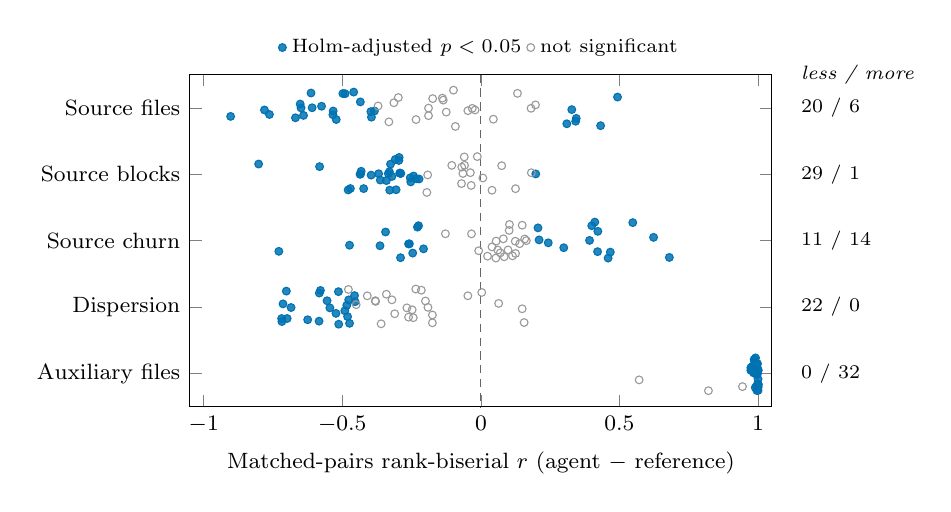
\begin{tikzpicture}
\begin{axis}[width=0.74\linewidth,height=58mm,xmin=-1.05,xmax=1.05,ymin=0.5,ymax=5.5,
 y dir=reverse,ytick={1,2,3,4,5},yticklabels={Source files,Source blocks,Source churn,Dispersion,Auxiliary files},xlabel={Matched-pairs rank-biserial $r$ (agent $-$ reference)},
 xtick={-1,-0.5,0,0.5,1},tick label style={font=\footnotesize},label style={font=\footnotesize},
 clip=false,legend style={font=\scriptsize,at={(0.5,1.02)},anchor=south,legend columns=2,draw=none}]
\addplot[only marks,mark=*,mark size=1.4pt,okblue,fill opacity=0.85] coordinates {(-0.490,0.787) (-0.649,1.001) (0.342,1.202) (-0.613,0.777) (-0.397,1.057) (0.344,1.159) (0.328,1.027) (-0.903,1.129) (-0.669,1.150) (-0.395,1.141) (-0.384,1.048) (-0.522,1.176) (-0.534,1.104) (-0.763,1.100) (0.493,0.838) (0.432,1.269) (0.310,1.240) (-0.459,0.763) (-0.435,0.911) (-0.781,1.032) (-0.575,0.976) (-0.640,1.114) (-0.652,0.943) (-0.533,1.048) (-0.609,0.999) (-0.498,0.785) (0.198,1.995) (-0.306,2.233) (-0.432,1.955) (-0.329,2.239) (-0.802,1.846) (-0.296,1.792) (-0.295,1.747) (-0.253,2.115) (-0.309,1.777) (-0.233,2.068) (-0.291,1.983) (-0.334,1.990) (-0.326,1.848) (-0.423,2.216) (-0.223,2.071) (-0.293,1.983) (-0.243,2.026) (-0.321,2.033) (-0.341,2.095) (-0.436,2.001) (-0.289,1.988) (-0.471,2.215) (-0.330,1.963) (-0.582,1.885) (-0.363,2.087) (-0.255,2.054) (-0.396,2.013) (-0.434,1.994) (-0.479,2.236) (-0.369,1.992) (0.467,3.172) (0.243,3.032) (-0.246,3.186) (0.400,2.775) (0.299,3.106) (-0.729,3.160) (0.459,3.262) (0.210,2.988) (-0.344,2.869) (-0.225,2.774) (0.623,2.950) (0.548,2.728) (0.411,2.720) (0.421,3.165) (0.422,2.859) (-0.474,3.068) (-0.290,3.256) (-0.364,3.076) (0.206,2.807) (-0.258,3.047) (0.680,3.252) (0.392,2.996) (-0.207,3.123) (-0.229,2.796) (-0.261,3.049) (-0.513,4.257) (-0.584,4.211) (-0.514,3.767) (-0.523,4.094) (-0.474,4.244) (-0.477,3.891) (-0.714,3.951) (-0.719,4.172) (-0.545,4.011) (-0.718,4.217) (-0.579,3.749) (-0.454,3.918) (-0.685,4.006) (-0.555,3.904) (-0.583,3.788) (-0.699,4.171) (-0.491,4.055) (-0.702,3.759) (-0.625,4.190) (-0.484,3.973) (-0.481,4.143) (-0.456,3.826) (0.990,5.212) (0.988,4.792) (0.996,5.017) (1.000,5.160) (0.996,5.009) (0.996,5.256) (0.987,4.810) (0.994,5.193) (1.000,4.938) (1.000,4.958) (0.974,4.952) (0.991,4.764) (0.979,4.891) (0.974,4.913) (0.996,4.868) (0.998,4.999) (1.000,5.157) (1.000,4.953) (0.987,4.982) (0.991,4.902) (0.984,4.990) (0.986,4.787) (1.000,5.166) (1.000,5.166) (1.000,5.177) (1.000,5.195) (0.998,4.850) (1.000,5.254) (1.000,5.212) (1.000,5.082) (0.977,4.948) (0.998,5.159)};
\addlegendentry{Holm-adjusted $p<0.05$}
\addplot[only marks,mark=o,mark size=1.4pt,okgrey] coordinates {(0.181,1.007) (-0.298,0.845) (-0.021,1.032) (-0.139,0.854) (-0.125,1.064) (0.132,0.782) (-0.234,1.177) (-0.371,0.972) (-0.174,0.861) (0.045,1.171) (-0.092,1.280) (-0.031,1.008) (-0.136,0.884) (-0.332,1.211) (-0.047,1.043) (-0.099,0.734) (-0.189,1.118) (-0.314,0.924) (0.197,0.956) (-0.189,1.004) (-0.070,2.140) (0.007,2.056) (-0.059,1.865) (-0.065,1.988) (-0.192,2.010) (-0.013,1.734) (0.125,2.217) (-0.038,1.976) (0.040,2.241) (-0.195,2.273) (-0.069,1.892) (-0.035,2.168) (0.075,1.871) (-0.060,1.739) (0.182,1.977) (-0.105,1.866) (0.055,3.006) (0.070,3.183) (0.114,3.228) (-0.034,2.897) (0.024,3.233) (0.124,3.008) (0.158,2.974) (0.054,3.261) (0.125,3.192) (0.103,2.756) (0.164,2.999) (0.098,3.139) (0.081,2.972) (0.140,3.045) (0.084,3.242) (0.149,2.767) (0.061,3.141) (0.040,3.094) (-0.128,2.896) (-0.008,3.151) (0.102,2.845) (-0.191,4.003) (-0.244,4.159) (0.156,4.232) (-0.410,3.830) (-0.235,3.728) (0.003,3.779) (-0.380,3.914) (-0.261,4.151) (-0.478,3.734) (-0.321,3.890) (-0.381,3.903) (-0.360,4.251) (-0.248,4.040) (-0.341,3.806) (-0.267,4.011) (-0.450,3.963) (-0.200,3.908) (-0.311,4.100) (0.064,3.944) (-0.047,3.829) (-0.175,4.236) (-0.215,3.745) (0.149,4.025) (-0.175,4.118) (0.944,5.196) (0.571,5.095) (0.821,5.258)};
\addlegendentry{not significant}
\draw[densely dashed,black!60] (axis cs:0,0.5) -- (axis cs:0,5.5);
\node[anchor=west,font=\scriptsize\itshape] at (axis cs:1.12,0.5) {less / more};
\node[anchor=west,font=\scriptsize] at (axis cs:1.12,1) {20 / 6};
\node[anchor=west,font=\scriptsize] at (axis cs:1.12,2) {29 / 1};
\node[anchor=west,font=\scriptsize] at (axis cs:1.12,3) {11 / 14};
\node[anchor=west,font=\scriptsize] at (axis cs:1.12,4) {22 / 0};
\node[anchor=west,font=\scriptsize] at (axis cs:1.12,5) {0 / 32};
\end{axis}
\end{tikzpicture}
%<<END:fig_rq1_effects>>
\caption{RQ1: per-system paired effects for 46 systems (22,048 non-empty pairs). Each point is one system. A negative $r$ means that the agent's patch is smaller or less dispersed than the reference patch for the same instance. Right margin: number of systems with a significant decrease / increase. A general directional claim requires 31 systems in one direction.}
\label{fig:rq1}
\end{figure}

Auxiliary files illustrate a scaffold confound. Thirty-two systems leave significantly more auxiliary files than the reference patches, which meets the threshold. This is the only metric for which H2 is formally supported. None of the 14 mini-swe-agent 2.0 systems shows the difference, whereas earlier scaffold versions can include exploratory or reproduction files when extracting the submission. Attributing this effect to model reasoning would therefore be misleading.

Location still carries information at the system level. Across systems, resolution rate correlates negatively with mean nonlocal edit share (Spearman $\rho=-0.83$) and positively with the share of patches that touch a reference file ($\rho=0.94$). The second association is partly expected, because resolved patches usually modify the defective code. An exploratory instance-clustered model estimates an odds ratio of 0.34 for resolution per unit increase in nonlocal share, after adjustment for system, source churn, and edited-file count. This association does not show that a nonlocal repair is wrong, and the running example is a concrete counterexample to that reading.

The available trajectories show broader recorded search than final edits. Among the seven execution-panel systems with published logs, the median number of referenced repository files ranges from one to six, whereas the median final edit touches at most one file. A referenced file is extracted from shell-command text and serves as a proxy for recorded exploration. It does not prove that the agent read or understood every file. A human reference patch supplies no comparable exploration history.

\paragraph{Answer to RQ1.}
In this scaffold family, agent patches tend to be smaller and less dispersed than reference patches, but no directional difference is general enough to meet the prespecified criterion. The data provide no evidence of a universal human--agent difference in repair locality. The motivation for edit-level evidence therefore cannot rest on patch breadth. RQ2 tests whether it rests on edit contribution instead.

\subsection{RQ2: What the counterfactual witnesses reveal}\label{sec:rq2}

The 1,674 reproduced patches contain 4,328 units. Twenty units receive \lab{X}, which leaves 4,308 conclusive classifications. Among the 3,394 conclusive agent units, 62.0\% are \lab{N}, 0.3\% are \lab{J}, 1.9\% are \lab{C}, and 35.9\% are \lab{U}. The 914 reference units are 64.1\% \lab{N}, 2.0\% \lab{C}, and 33.9\% \lab{U}, with no \lab{J} units. These categories describe the selected witness and observed full-patch withdrawals, not global semantic necessity.

Among source units, 1,093 of 3,206 conclusive agent units are removable (34.1\%), against 328 of 914 reference units (35.9\%). The difference is $-1.8$ percentage points, with a 95\% interval of $[-8.6, 6.1]$. At least one removable unit of any kind appears in 30.1\% of agent patches (interval $[26.2\%, 34.0\%]$) and in 25.4\% of reference patches ($[20.7\%, 30.5\%]$). The pooled comparison mixes instance populations, because each system resolves a different subset of instances. Figure~\ref{fig:rq2} therefore compares each system with the reference patches of the instances it resolved. On those instances the reference share varies from 12.8\% (Qwen2.5-Coder) to 38.2\% (Claude 4.6 Opus), so instance composition alone moves the baseline substantially. DeepSeek V3.2 retains a higher removable share than its matched references ($+11.6$ points, $[4.3, 20.5]$, Holm $p=0.003$). GPT-4o shows a similar unadjusted difference ($+19.3$, $[4.4, 32.9]$, Holm $p=0.06$). The intervals of the remaining six systems include zero, and four of them point below the reference. The pooled matched difference is $-3.3$ points ($[-10.3, 5.4]$).

\begin{figure}[pos=htbp]
\centering
%<<GEN:fig_rq2_matched>>
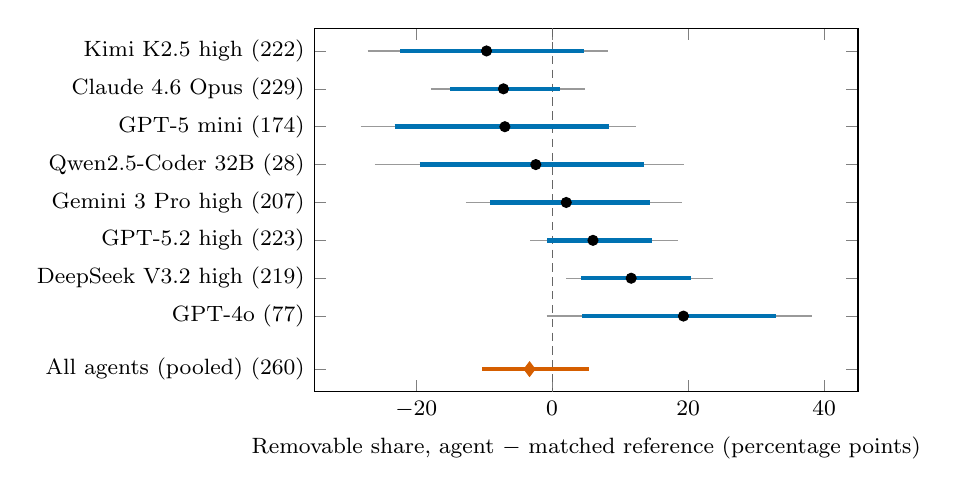
\begin{tikzpicture}
\begin{axis}[width=0.70\linewidth,height=62mm,xmin=-35,xmax=45,ymin=0.4,ymax=10.0,y dir=reverse,
 ytick={1,2,3,4,5,6,7,8,9.4},yticklabels={{Kimi K2.5 high (222)},{Claude 4.6 Opus (229)},{GPT-5 mini (174)},{Qwen2.5-Coder 32B (28)},{Gemini 3 Pro high (207)},{GPT-5.2 high (223)},{DeepSeek V3.2 high (219)},{GPT-4o (77)},{All agents (pooled) (260)}},xlabel={Removable share, agent $-$ matched reference (percentage points)},
 tick label style={font=\footnotesize},label style={font=\footnotesize},clip=false]
\draw[densely dashed,black!60] (axis cs:0,0.4) -- (axis cs:0,10.0);
\draw[okgrey,line width=0.5pt] (axis cs:-27.16,1) -- (axis cs:8.24,1);
\draw[okgrey,line width=0.5pt] (axis cs:-17.82,2) -- (axis cs:4.86,2);
\draw[okgrey,line width=0.5pt] (axis cs:-28.16,3) -- (axis cs:12.30,3);
\draw[okgrey,line width=0.5pt] (axis cs:-26.09,4) -- (axis cs:19.34,4);
\draw[okgrey,line width=0.5pt] (axis cs:-12.69,5) -- (axis cs:19.13,5);
\draw[okgrey,line width=0.5pt] (axis cs:-3.19,6) -- (axis cs:18.51,6);
\draw[okgrey,line width=0.5pt] (axis cs:2.07,7) -- (axis cs:23.62,7);
\draw[okgrey,line width=0.5pt] (axis cs:-0.82,8) -- (axis cs:38.19,8);
\draw[okblue,line width=1.6pt] (axis cs:-22.35,1) -- (axis cs:4.62,1);
\draw[okblue,line width=1.6pt] (axis cs:-15.04,2) -- (axis cs:1.23,2);
\draw[okblue,line width=1.6pt] (axis cs:-23.17,3) -- (axis cs:8.36,3);
\draw[okblue,line width=1.6pt] (axis cs:-19.51,4) -- (axis cs:13.56,4);
\draw[okblue,line width=1.6pt] (axis cs:-9.11,5) -- (axis cs:14.46,5);
\draw[okblue,line width=1.6pt] (axis cs:-0.74,6) -- (axis cs:14.76,6);
\draw[okblue,line width=1.6pt] (axis cs:4.32,7) -- (axis cs:20.50,7);
\draw[okblue,line width=1.6pt] (axis cs:4.41,8) -- (axis cs:32.87,8);
\addplot[only marks,mark=*,mark size=1.8pt,black] coordinates {(-9.65,1) (-7.16,2) (-6.95,3) (-2.40,4) (2.08,5) (6.01,6) (11.63,7) (19.32,8)};
\draw[okverm,line width=1.6pt] (axis cs:-10.28,9.4) -- (axis cs:5.41,9.4);
\addplot[only marks,mark=diamond*,mark size=2.6pt,okverm] coordinates {(-3.32,9.4)};
\end{axis}
\end{tikzpicture}
%<<END:fig_rq2_matched>>
\caption{RQ2: difference in removable share of conclusive source units between each system and the reference patches of the same instances (number of instances in parentheses). Thick bars: 95\% instance-cluster bootstrap intervals. Thin grey bars: Bonferroni-adjusted intervals across eight systems. Diamond: all agent units against the reference units of the 260 instances with at least one agent unit.}
\label{fig:rq2}
\end{figure}

Removable edits are thus common in both populations, and their prevalence depends more on the system and instance than on whether the author is human or agent. Passing-patch acceptance leaves the edit-level question open for all of them.

All 49 conclusive agent test-file units and 139 auxiliary-file units are removable under the benchmark obligations. This result reflects the harness, which protects its own test patch, and reproduction scripts typically lie outside the tested execution path. It does not imply that developer-written tests or debugging scripts have no engineering value.

Table~\ref{tab:comparisons} reports how well cheaper signals approximate the operational roles. Reference-file overlap flags removable edits with precision 0.83 but recall only 0.27. Of the 1,093 removable source units, 797 lie inside reference-edited files. Conversely, 60 retained source units lie outside those files, and the reference-file rule rejects all of them. Import proximity retains 63\% of these nonlocal retained units but finds only 21\% of removable units. Location therefore provides useful evidence but fails to distinguish many edits within the same repair area.

What do removable edits look like? A rule-based classification of each unit's changed lines (\nolinkurl{analysis/revision/v2_checks.py}) gives a partial answer. Removable agent source units are small (median two changed lines, against three for retained units). They are more often purely non-behavioral, changing only comments, docstring delimiters, imports, or whitespace (15.8\% against 4.5\% of retained units). They also more often resemble another edit that the witness retains: 28.8\% have a textual similarity of at least 0.6 to a retained unit, against 18.8\% of retained units, and 69.4\% lie in a file that also contains a retained unit. Added conditionals or exception handling are \emph{less} common among removable units (31.0\%) than among retained ones (40.1\%). Most removable units (53.2\%) are ordinary code changes that the classification does not separate further. Reference patches show the same tendencies, with even fewer added conditionals among their removable units (8.5\%). The rules are deliberately conservative and measure form, not purpose. Whether a removable edit is redundant, defensive, or valuable for an untested requirement requires manual inspection.

\begin{table}[pos=htbp]
\caption{Agreement with counterfactual roles for conclusive agent source units. Precision and recall concern removable units. Coverage is the share of 3,206 units with a parsed aggregate prediction. Intervals are 95\% instance-cluster intervals for MCC. The reference-file rule has privileged access to the reference patch. The first five judges aggregate three seeds; the additional judges use a single seed.}
\label{tab:comparisons}
\centering\small
\begin{tabular}{lrrrrl}
\toprule
Method & Coverage & Precision & Recall & F1 & MCC [interval] \\
\midrule
Reference-file & 100\% & .83 & .27 & .41 & .37 [.26, .46] \\
Issue-mention & 100\% & .40 & .63 & .49 & .14 [.03, .24] \\
Import-proximity & 100\% & .91 & .21 & .34 & .35 [.24, .44] \\
All-retained & 100\% & -- & .00 & -- & -- \\
\midrule
Gemma 2 9B & 99.8\% & .77 & .16 & .27 & .25 [.19, .33] \\
Llama 3.1 8B & 98.3\% & .36 & .33 & .35 & .03 [$-$.05, .11] \\
Mistral Small 24B & 100\% & .91 & .29 & .44 & .42 [.34, .49] \\
Phi-4 14B & 98.5\% & .93 & .21 & .35 & .37 [.29, .44] \\
Qwen2.5-Coder 7B & 99.8\% & .52 & .37 & .43 & .22 [.13, .31] \\
\midrule
\multicolumn{6}{l}{\emph{Additional judges, one seed, run after the main analysis}} \\
Devstral 24B & 98.5\% & .96 & .27 & .42 & .43 [.35, .50] \\
GPT-OSS 20B & 100\% & .91 & .20 & .33 & .34 [.26, .44] \\
Qwen3-Coder 30B & 95.9\% & .91 & .22 & .36 & .37 [.30, .45] \\
\bottomrule
\end{tabular}
\end{table}

Within the main panel, the best judge MCC is 0.42, for Mistral Small. Mistral Small and Phi-4 are precise when they predict removability, but their recall is only 0.29 and 0.21. The issue-mention rule has a higher F1 than any judge, although its MCC is lower. These metrics capture different tradeoffs and do not support a blanket claim that LLM judges outperform location. Under the prespecified rule, H3 is not supported. The reference-file rule meets both conditions: it retains none of the 60 nonlocal needed units, and its F1 (0.41) is below the best judge's (0.44). The issue-mention rule fails the F1 condition (0.49), and import proximity fails the retention condition, keeping 63\% of the nonlocal needed units. Location rules therefore do not uniformly underperform the judges. Both families fall well short of the counterfactual labels. A matched exploratory comparison tests whether judges were handicapped by not seeing the goal tests. It uses the same seed and units parsed in both variants. The test information raises MCC for Phi-4 ($+0.07$, $[0.01, 0.15]$) and Qwen2.5-Coder ($+0.15$, $[0.02, 0.27]$), but not for Mistral Small ($-0.01$, $[-0.06, 0.03]$), Gemma, or Llama. The best informed MCC is 0.45. Test names and test code thus help weaker judges without closing the gap to the counterfactual measurement. Three further judges, run after the main analysis with the same prompts and decoding on one seed, do not change this picture either. All three are precise but conservative, like Phi-4. Devstral 24B, an agentic coding model, is the strongest (precision 0.96, recall 0.27, F1 0.42, MCC 0.43 [0.35, 0.50]). GPT-OSS 20B, a reasoning model, and Qwen3-Coder 30B, a larger code model, reach MCC 0.34 [0.26, 0.44] and 0.37 [0.30, 0.45] with recall 0.20 and 0.22. None reaches Mistral Small on the same single seed, where Mistral Small scores F1 0.50 and MCC 0.46. The lower coverage of Qwen3-Coder (95.9\%) comes from responses that omit some units. The H3 decision is unchanged, because the best judge F1 remains Mistral Small's 0.44.

\paragraph{Answer to RQ2.}
Counterfactual witnesses identify a substantial removable portion of the tested patches, including many source edits inside reference-edited files. The removable share does not differ detectably between pooled agent and reference patches. It varies between systems, and one system exceeds its matched references after adjustment. Location heuristics and judges approximate the measurement only partly, even with test information or larger judge models. The result establishes a gap in evidence about edit contribution. It does not establish that removable edits are incorrect, or that the phenomenon is specific to agents.

\subsection{RQ3: Additional preservation evidence}\label{sec:rq3}

The selector finds an envelope for 1,636 valid patches and none for 38. The median nonempty envelope contains 104 tests observed to pass on the base. Confirmed reference-filtered envelope failures occur in 19 of 1,346 agent patches with nonempty envelopes (1.4\%, interval $[0.4\%, 2.7\%]$). In ten cases, add-back observations associate a failure with omitted units. In nine cases, the failure persists in the reduced witness, which shows that the core obligations permit a change that the envelope questions.

The records also contain two envelope signals for reference patches. A reference patch compared against its own reference-filtered baseline should not yield a stable difference. These signals point to repeated-execution effects, missing test reports, or baseline caching. They are not evidence of agent-specific regressions, and they caution against treating every envelope signal as a confirmed semantic defect. Re-execution reduces such uncertainty but cannot make the oracle complete.

Figure~\ref{fig:rq3} reports the controlled probes. Official tests detect 78 of 249 evaluable semantic probes (31.3\%, interval $[25.7\%, 37.3\%]$). The envelope detects another 25, which raises combined detection to 41.4\% ($[35.3\%, 47.4\%]$). The paired gain is 10.0 percentage points ($[6.4, 14.1]$), and all 25 discordant probes favor the envelope (exact McNemar $p<10^{-7}$). The remaining 146 semantic probes (58.6\%) are detected by neither. Detection depends strongly on the operator. Condition negation reaches 57.4\% combined detection, whereas integer perturbation reaches only 10.9\%, with one probe detected by the official tests and four more by the envelope. No neutral probe produced a test signal.

\begin{figure}[pos=htbp]
\centering
%<<GEN:fig_rq3_ops>>
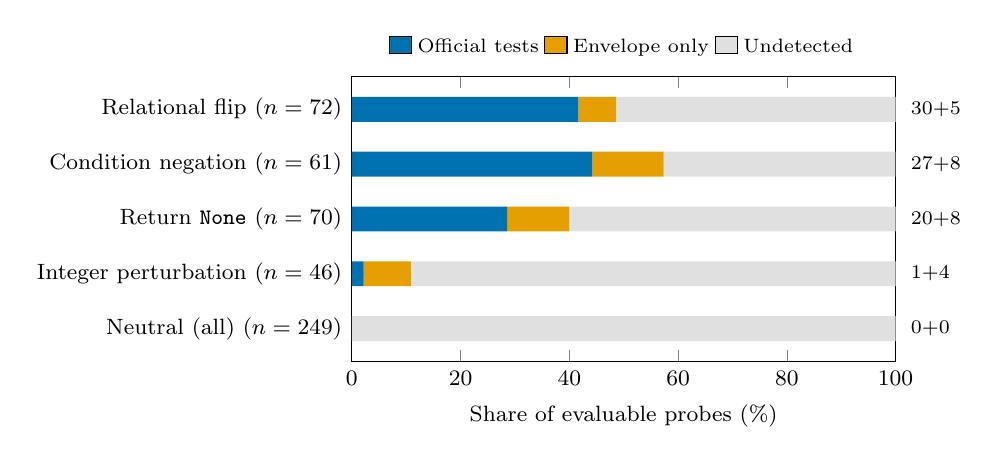
\begin{tikzpicture}
\begin{axis}[xbar stacked,bar width=9pt,width=0.70\linewidth,height=52mm,xmin=0,xmax=100,
 ymin=0.4,ymax=5.6,y dir=reverse,ytick={1,2,3,4,5},yticklabels={{Relational flip ($n=72$)},{Condition negation ($n=61$)},{Return \code{None} ($n=70$)},{Integer perturbation ($n=46$)},{Neutral (all) ($n=249$)}},
 xlabel={Share of evaluable probes (\%)},tick label style={font=\footnotesize},label style={font=\footnotesize},
 legend style={font=\scriptsize,at={(0.5,1.03)},anchor=south,legend columns=3,draw=none},clip=false]
\addplot[fill=okblue,draw=none] coordinates {(41.67,1) (44.26,2) (28.57,3) (2.17,4) (0.00,5)};
\addlegendentry{Official tests}
\addplot[fill=okorange,draw=none] coordinates {(6.94,1) (13.11,2) (11.43,3) (8.70,4) (0.00,5)};
\addlegendentry{Envelope only}
\addplot[fill=black!12,draw=none] coordinates {(51.39,1) (42.62,2) (60.00,3) (89.13,4) (100.00,5)};
\addlegendentry{Undetected}
\node[anchor=west,font=\scriptsize] at (axis cs:101,1) {30+5};
\node[anchor=west,font=\scriptsize] at (axis cs:101,2) {27+8};
\node[anchor=west,font=\scriptsize] at (axis cs:101,3) {20+8};
\node[anchor=west,font=\scriptsize] at (axis cs:101,4) {1+4};
\node[anchor=west,font=\scriptsize] at (axis cs:101,5) {0+0};
\end{axis}
\end{tikzpicture}
%<<END:fig_rq3_ops>>
\caption{RQ3: outcomes of injected probes by operator. Right margin: probes detected by official tests + additionally detected by the envelope. Detection means an observed test signal for a mutation probe, not independently established detection of a genuine fault. One erroneous execution per category is excluded.}
\label{fig:rq3}
\end{figure}

Zero observed neutral failures do not establish a zero population false-positive rate; with 249 probes, the one-sided 95\% upper bound is 1.2\%. Nor can every undetected semantic mutation be counted as a missed real fault without an independent behavioral witness. The measured quantity is sensitivity to the stated operator distribution and the selected sites. Integer perturbations, in particular, often change constants whose exact value no test constrains. A stronger study would distinguish killable faults, equivalent mutations, and mutations whose affected behavior lies outside the intended contract.

\paragraph{Answer to RQ3.}
Additional selected tests reveal behavior changes beyond the official obligations, with a statistically clear but modest gain. Most semantic probes remain undetected, particularly value perturbations, and add-back associations require contextual interpretation. A removable label must therefore remain relative to its contract and cannot serve as a certificate of harmlessness.

\subsection{RQ4: Cost, edit interaction, and reduction quality}\label{sec:rq4}

\paragraph{Cost.}
Core triage uses a median of three oracle executions per valid patch, with a 90th percentile of 11. Of the 1,674 patches, 877 contain one unit and another 376 contain two, so the overall median is dominated by small patches. Figure~\ref{fig:rq4} shows how executions grow with unit count (Spearman $\rho=0.97$). The median rises from 3 for one unit to 25 for 9--16 units and 66 for 17 or more, with a maximum of 256. The precheck rejects 79 configurations without a core test run. Across all valid patches, the median recorded wall time is 38.7 seconds. That timer starts before container execution and stops after optional ablations and the envelope. The timing values therefore do not establish a cost for the complete proposed workflow, or that one minimization method is faster than another under equal work.

\begin{figure}[pos=htbp]
\centering
%<<GEN:fig_rq4_cost>>
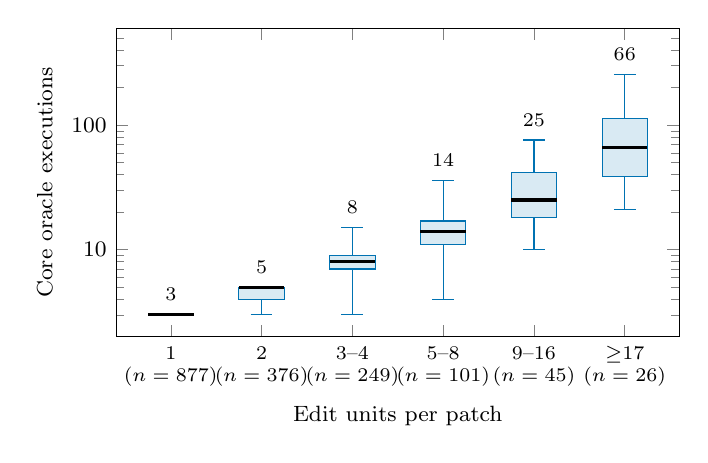
\begin{tikzpicture}
\begin{semilogyaxis}[width=0.72\linewidth,height=55mm,xmin=0.4,xmax=6.6,ymin=2,ymax=600,
 xtick={1,2,3,4,5,6},xticklabels={{1\\($n=877$)},{2\\($n=376$)},{3--4\\($n=249$)},{5--8\\($n=101$)},{9--16\\($n=45$)},{$\geq$17\\($n=26$)}},
 xticklabel style={align=center,font=\scriptsize},yticklabel style={font=\footnotesize},
 xlabel={Edit units per patch},ylabel={Core oracle executions},label style={font=\footnotesize},
 log ticks with fixed point,clip=false]
\addplot[draw=none] coordinates {(1,3)};
\draw[okblue] (axis cs:1,3) -- (axis cs:1,3);
\draw[okblue] (axis cs:1,3) -- (axis cs:1,3);
\draw[okblue] (axis cs:0.88,3) -- (axis cs:1.12,3);
\draw[okblue] (axis cs:0.88,3) -- (axis cs:1.12,3);
\draw[okblue,fill=okblue!15] (axis cs:0.75,3) rectangle (axis cs:1.25,3);
\draw[black,line width=1.2pt] (axis cs:0.75,3) -- (axis cs:1.25,3);
\node[font=\scriptsize,anchor=south] at (axis cs:1,3.24) {3};
\draw[okblue] (axis cs:2,3) -- (axis cs:2,4);
\draw[okblue] (axis cs:2,5) -- (axis cs:2,5);
\draw[okblue] (axis cs:1.88,3) -- (axis cs:2.12,3);
\draw[okblue] (axis cs:1.88,5) -- (axis cs:2.12,5);
\draw[okblue,fill=okblue!15] (axis cs:1.75,4) rectangle (axis cs:2.25,5);
\draw[black,line width=1.2pt] (axis cs:1.75,5) -- (axis cs:2.25,5);
\node[font=\scriptsize,anchor=south] at (axis cs:2,5.4) {5};
\draw[okblue] (axis cs:3,3) -- (axis cs:3,7);
\draw[okblue] (axis cs:3,9) -- (axis cs:3,15);
\draw[okblue] (axis cs:2.88,3) -- (axis cs:3.12,3);
\draw[okblue] (axis cs:2.88,15) -- (axis cs:3.12,15);
\draw[okblue,fill=okblue!15] (axis cs:2.75,7) rectangle (axis cs:3.25,9);
\draw[black,line width=1.2pt] (axis cs:2.75,8) -- (axis cs:3.25,8);
\node[font=\scriptsize,anchor=south] at (axis cs:3,16.2) {8};
\draw[okblue] (axis cs:4,4) -- (axis cs:4,11);
\draw[okblue] (axis cs:4,17) -- (axis cs:4,36);
\draw[okblue] (axis cs:3.88,4) -- (axis cs:4.12,4);
\draw[okblue] (axis cs:3.88,36) -- (axis cs:4.12,36);
\draw[okblue,fill=okblue!15] (axis cs:3.75,11) rectangle (axis cs:4.25,17);
\draw[black,line width=1.2pt] (axis cs:3.75,14) -- (axis cs:4.25,14);
\node[font=\scriptsize,anchor=south] at (axis cs:4,38.88) {14};
\draw[okblue] (axis cs:5,10) -- (axis cs:5,18);
\draw[okblue] (axis cs:5,42) -- (axis cs:5,76);
\draw[okblue] (axis cs:4.88,10) -- (axis cs:5.12,10);
\draw[okblue] (axis cs:4.88,76) -- (axis cs:5.12,76);
\draw[okblue,fill=okblue!15] (axis cs:4.75,18) rectangle (axis cs:5.25,42);
\draw[black,line width=1.2pt] (axis cs:4.75,25) -- (axis cs:5.25,25);
\node[font=\scriptsize,anchor=south] at (axis cs:5,82.08) {25};
\draw[okblue] (axis cs:6,21) -- (axis cs:6,38.75);
\draw[okblue] (axis cs:6,113.25) -- (axis cs:6,256);
\draw[okblue] (axis cs:5.88,21) -- (axis cs:6.12,21);
\draw[okblue] (axis cs:5.88,256) -- (axis cs:6.12,256);
\draw[okblue,fill=okblue!15] (axis cs:5.75,38.75) rectangle (axis cs:6.25,113.25);
\draw[black,line width=1.2pt] (axis cs:5.75,66) -- (axis cs:6.25,66);
\node[font=\scriptsize,anchor=south] at (axis cs:6,276.48) {66};
\end{semilogyaxis}
\end{tikzpicture}
%<<END:fig_rq4_cost>>
\caption{RQ4: core oracle executions per patch by number of edit units (log scale; box: interquartile range; whiskers: minimum and maximum; label: median). Executions include the two full-patch runs and the base run.}
\label{fig:rq4}
\end{figure}

\paragraph{Interactions.}
The records contain 82 \lab{C} units in 43 patches and nine \lab{J} units in seven patches. In these cases the full-patch single-withdrawal view and the selected passing witness disagree. A procedure that treated every failed single withdrawal as global necessity would keep the omitted withdrawal-sensitive edits. These observations motivate reporting both the full-patch experiment and the reduced witness.

\paragraph{Reduction quality.}
For the 1,603 patches with at most eight units, an ablation searched exhaustively for minimum-cardinality closed configurations. Our first comparison found the exhaustive minimum larger than a known passing witness in four records, which is impossible for a correct exhaustive search under a deterministic oracle. An audit traced the cause to the baseline, not to \tool{}. The baseline enumerated subsets by their size before closure. A small generator whose closure was large, such as two units whose closure was the whole patch, was returned before a smaller valid closed set was reached. All four records contain requires edges, and in each the smaller \tool{} witness had itself been observed valid. We corrected the enumeration to order closed configurations by their own size and added regression and property-based tests. The original code fails the regression case and 9 of the 40 random cases. We then re-derived the minimum from the recorded outcomes. For 1,595 records, every closed configuration smaller than the witness has a recorded or static-precheck non-valid outcome. For seven records, 31 smaller closed configurations had never been executed. We executed them, together with one re-execution of each witness. All 31 failed and all seven witnesses passed again. One record (\code{sympy__sympy-19783}, Kimi K2.5) has a valid two-unit closed configuration, whereas \tool{}'s witness has three units. This is the expected gap between withdrawal minimality and minimum cardinality. Overall, 1,602 of 1,603 witnesses (99.9\%) have minimum cardinality among closed configurations. Matching size establishes neither uniqueness of the minimal repair nor stability of every edit label.

These conclusions assume deterministic outcomes, which we checked directly. The records execute 3,746 configurations more than once, through repeated full-patch checks and ablation reruns. Two of them, in \code{django__django-16263} (reference) and \code{sympy__sympy-13091} (Kimi K2.5), produced conflicting outcomes. Both patches have more than eight units, and their labels inherit that instability. Nondeterminism is therefore rare (0.05\% of repeated configurations) but present.

\paragraph{Ablations and a TRIM-style baseline.}
Every multi-unit patch also recorded three reduction ablations, and we added a diff-only reimplementation of TRIM's search~\citep{mathai2026trim}. TRIM has no public artifact, and the bash-only submissions do not record agent edits in a replayable form, so its trajectory-derived edit sequences are unavailable. The reimplementation keeps TRIM's search: it visits edit groups in reverse order, first by file and then by edit unit, keeps a removal when the remaining patch still passes, and repeats each level to a fixpoint. It uses neither the requires closure nor the syntax precheck. All strategies query the same oracle. A configuration observed earlier in the campaign is counted once per strategy and reused, and the 1,091 configurations that only the TRIM-style search reached were newly executed (three timed out and count as unknown). Table~\ref{tab:ablation} compares the strategies on the 797 patches with at least two units. The counts measure search work under one oracle; they exclude the base run, repeated full-patch runs, and the leave-one-out withdrawals, which \tool{} needs for its roles (3,246 executions).

\begin{table}[pos=htbp]
\caption{Reduction strategies on the 797 valid patches with at least two units. ``Executions'' counts distinct configurations sent to the test oracle; ``syntax-invalid'' counts configurations that fail to parse but would be executed. ``Not closed'' means the result retains a unit without a unit it requires under $R$; in parentheses, results that pyflakes flags with an undefined name that the full patch does not have.}
\label{tab:ablation}
\centering\small
\begin{tabular}{lrrrrr}
\toprule
Strategy & Executions & $\geq$17 units & Syntax-invalid & Not closed & Same witness \\
\midrule
Plain \textsc{ddmin} & 6,397 & 1,806 & 47 & 33 & 764 \\
\textsc{ddmin} + precheck & 6,267 & 1,766 & 0 & 33 & 764 \\
Dependency-aware \textsc{ddmin} (\tool{}) & 5,437 & 1,578 & 77$^{a}$ & 0 & 797 \\
TRIM-style, diff-only & 4,482 & 823 & 34 & 32 (3) & 752 \\
\bottomrule
\end{tabular}

\smallskip{\footnotesize $^{a}$ In \tool{}, which combines closure with the precheck, these configurations are rejected without execution.}
\end{table}

Dependency closure saves 15\% of the executions of plain \textsc{ddmin} (26\% on the 363 patches with requires edges). It also prevents the 33 unclosed results that plain reduction returns. The precheck removes every execution of an unparsable variant. The TRIM-style search is cheaper still, by 18\% overall and by almost half on the 26 patches with at least 17 units, where its coarse file-level pass removes many units at once. The two methods agree on the witness in 752 patches (94.4\%). The TRIM-style witness is larger in 13 patches, where removing one group at a time misses a removal that only a joint change permits. It is smaller in 30. One of these is the \code{sympy__sympy-19783} case discussed above. In the other 29 it retains a unit without a unit that \tool{}'s relation says it requires. In 3 of the 29, pyflakes reports a new undefined name, so the passing witness hides a latent failure on an untested path. In the remaining 26, the relation is conservative. Inspection shows two causes: function-local names that are assigned in several units, and same-named methods defined in several classes. Both are matched at module scope and therefore link unrelated units. The exhaustive-search result above holds for configurations closed under this relation. A function-scoped relation would recover these smaller witnesses.

\paragraph{Answer to RQ4.}
Core counterfactual execution is inexpensive for the predominantly small patches in this sample and grows steeply for large ones. Dependency closure and the syntax precheck reduce the work of delta debugging and prevent unclosed or unparsable variants. A diff-only TRIM-style search is cheaper on large patches and returns the same witness in 94\% of cases. Its smaller witnesses mostly expose an over-approximating requires relation rather than an error of \tool{}. A few rely on an undefined name. Interaction cases justify evidence beyond leave-one-out. Although \tool{} guarantees only withdrawal minimality, its witnesses attain minimum cardinality in all but one of 1,603 exhaustively checked patches. The existing timing instrumentation does not isolate end-to-end governance cost.

\subsection{Planned evaluation of the contract workflow}\label{sec:future}

The implemented analysis does not establish the benefits of a DSL or of integrating evidence into agent development. We propose three complementary studies. Each has a primary outcome and a result that would weaken the proposed approach. These studies are future work, not completed experiments.

\paragraph{Study A: language value and contract fidelity.}
Compare natural-language instructions, an equivalent structured YAML configuration, and \dsl{} in a balanced crossover design with software developers. Each participant writes and amends goal and preservation policies for different tasks under each interface. An expert-authored mapping from requirements to tests, prepared before the sessions, serves as the reference. The primary outcome is the rate of contracts that express all required obligations without adding contradictory ones. Secondary outcomes are authoring time, diagnostic recovery, comprehension, and amendment errors. A pilot estimates variance to set the confirmatory sample size for a prespecified effect or interval width. A null advantage over equivalent YAML would weaken the claim that dedicated syntax improves governance, while leaving the underlying contract model useful.

\paragraph{Study B: equal-budget analysis and review.}
RQ4 already compares the reduction strategies, including a diff-only TRIM-style search, on the existing patches under one oracle. The remaining comparison needs the original tool and trajectories. Freeze a new task set and its candidate patches before any tuning. Compare unchanged patches, leave-one-out, dependency-aware \textsc{ddmin}, a structure-aware reducer, TRIM, and \tool{}. TRIM is the most important comparison because it also uses counterfactual execution and reports about half the validation cost of delta debugging~\citep{mathai2026trim}. Supply trajectories where available and report a separate diff-only stratum where they are not. Use identical analyzer-visible tests, clean environments, and equal test-execution or wall-time budgets. Measure witness size, retained held-out behavior, unresolved outcomes, and total execution cost, and evaluate attribution evidence separately from plain minimization. This design can reveal whether the added evidence is worth its cost, rather than assuming that a richer report is better.

For independent preservation assessment, prepare evaluation-only tests or adjudicated behavioral checks that the analyzer cannot access. Keep reference-patch information out of the deployed method and use it only for explicitly privileged diagnostics. Independent reviewers inspect a stratified sample of retained, omitted, and unresolved units with the issue context. A blinded crossover review task then compares ordinary diffs with the evidence report. The primary review outcome is correct acceptance or rejection under an adjudicated requirement set. Review time is secondary, because a faster incorrect decision is not an improvement. If reduced patches lose held-out behavior or the evidence increases confident review errors, the workflow must be revised.

\paragraph{Study C: cumulative development and wider applicability.}
Use the version-pinned benchmark roles in Table~\ref{tab:benchmarks}. SWE-bench Verified remains the primary repair benchmark because it supplies repository tasks, reproducible environments, and archived candidate patches. Defects4J provides a Java replication setting~\citep{just2014defects4j}, for which the dependency model must be adapted and validated rather than transferred mechanically from Python. SlopCodeBench supplies successive specification updates for studying how earlier agent changes affect later development~\citep{orlanski2026slopcodebench}. Its exact release must be frozen, because the paper and repository have changed across versions.

In the iterative study, each accepted implementation is carried into the next task. Compare ordinary agent iteration with contract-and-evidence feedback under matched generation and validation budgets, and hold later checkpoint tests out of earlier feedback. The primary outcome is successful completion of subsequent requirements while preserving prior required behavior. Secondary outcomes include repair churn, redundant structure, new contract obligations, and cumulative execution cost. If a smaller initial patch makes later changes harder, that would challenge minimality as a review objective.

\begin{table}[pos=htbp]
\caption{Recommended benchmark roles for the remaining evaluation. Only the SWE-bench Verified execution subset has been analyzed in the results reported here.}
\label{tab:benchmarks}
\centering\small
\begin{tabularx}{\linewidth}{lXXX}
\toprule
Benchmark & Why it fits & Required preparation & Main limitation \\
\midrule
SWE-bench Verified & Real issue repair, candidate patches, executable obligations & Freeze snapshots; audit environments and hidden evaluation split & Public tests and reference history may be contaminated \\
Defects4J & Reproducible real Java faults and regression suites & Obtain agent candidates; validate Java unit dependencies & Curated human fixes alone do not test agent behavior \\
SlopCodeBench & Repeated implementation under evolving requirements & Freeze release; preserve trajectories; hide future tests & Different task construct from repository bug repair \\
\bottomrule
\end{tabularx}
\end{table}

All three studies should report information access, failures, model and scaffold versions, and full denominators. A contract-generated test and a held-out evaluator test must not silently become the same evidence source. A question counts as answered only when its stated construct has been measured, not merely because a benchmark score improves.

\subsection{Discussion}\label{sec:discussion}

\paragraph{The deeper problem is an evidence mismatch.}
The starting intuition was that an agent may analyze and repair software differently from a particular human developer. The data support a narrower and more useful conclusion: neither a reference repair location nor a passing whole patch establishes the contribution of every candidate edit. RQ1 finds no general breadth difference in this sample, and RQ2 finds many removable edits inside reference-edited files. Governance based only on edit radius would miss those cases. Governance based on explicit obligations asks the relevant question without requiring a cognitive theory of agents.

\paragraph{Why counterfactual witnesses succeed where cheaper signals fail.}
Location proxies and judges observe where an edit is and what it looks like. A withdrawal experiment observes what happens without the edit. Most removable source edits lie in the same files as the reference repair (797 of 1,093), and most share a file with a retained edit. Many are small, non-behavioral, or textually similar to a retained edit (RQ2), so file-level location cannot separate them from the effective change. Test information helps some judges (RQ2), which suggests that their errors partly reflect missing knowledge of the obligations. Even informed judges reach an MCC below 0.5, however, so predicting execution outcomes from text remains hard. The counterfactual witness is more expensive, but RQ4 shows that the expense is small for typical patches.

\paragraph{Human patches expose the oracle's limits.}
Reference and agent patches show similar pooled source-unit removability, which rules out an agent-specific interpretation of the overall result. The system-level differences show that some agent configurations leave more removable code than the corresponding human fixes, while others leave less. Maintainers may add symmetric fixes, defensive branches, and readability improvements that the benchmark does not exercise; three in four removable reference units are ordinary code changes rather than comments, imports, or whitespace. An analyzer that calls these units removable may describe the test suite accurately but the engineering task incompletely. This is why the reference comparison matters: it shows that relevance cannot be defined solely by human location or by test necessity.

\paragraph{Alternative repair routes deserve evidence, not automatic rejection.}
Location is informative across systems, but it is not a correctness rule for an individual repair. The running example demonstrates a nonlocal route that passes the obligations, with both retained and omitted edits along that route. A behavioral contract admits that possibility. Counterfactual success does not, however, excuse a design that violates an untested requirement. The appropriate response is to make that requirement explicit and gather more evidence.

\paragraph{Preservation signals should drive refinement, not certification.}
The envelope's additional detections show why reduction and preservation checks belong together. The large undetected fraction, concentrated in value perturbations, shows why they are insufficient as a safety claim. A failure in the reduced witness calls for stronger obligations or a revised repair. A failure associated with omitted units focuses review on those groups. The proposed report should make both cases visible, including tests excluded by the retrospective reference rule.

\paragraph{Relation to trajectory-based minimization.}
TRIM already studies execution-based removal of residual agent changes and reports substantial reductions at about half the validation cost of delta debugging~\citep{mathai2026trim}. Counterfactual patch minimization is therefore not new. Our RQ4 results put the two approaches side by side under one oracle, without trajectories. TRIM's reverse, coarse-to-fine search is the cheaper minimizer, especially for large patches, and its witnesses agree with \tool{}'s in 94\% of patches. Where they differ, both methods have a characteristic weakness. A search without a dependency model can return a passing patch that relies on an undefined name. A conservative name-based dependency model can keep units the tests do not need. Trajectory order and a scoped relation are therefore complementary, and \tool{}'s evidence model could adopt TRIM's search order for its reduction step. The distinct elements of \tool{} are the explicit behavioral contract, the separation of contextual roles from global necessity, and preservation observations attached to omitted groups. TRIM also reports that agent code tends to be larger than human code, whereas our RQ1 finds no general difference. The constructs differ in scaffolds, tasks, and size measures, so the two results do not directly contradict each other. Our comparison uses a reimplementation and no trajectories, so it does not evaluate TRIM as published. Whether the additional evidence improves development outcomes also remains an empirical question, which Study~B makes falsifiable.

\paragraph{Auditing a baseline is part of the evidence.}
The exhaustive-search defect shows how a reduction comparison can fail silently once a dependency closure is involved. The faulty baseline agreed with \tool{} in 99.7\% of records and disagreed only where requires edges existed. Without the audit, these disagreements would have read as either a flaw in \tool{} or an unexplained anomaly. Generators and their closures are easy to conflate, and the same pitfall applies to any closure-aware reduction. Evaluations of such methods should check their baselines against brute-force enumeration over closed sets.

\paragraph{A review aid is not an automatic merge policy.}
The most defensible near-term use is to expose a passing repair core and the evidence for omitted groups. A maintainer may retain additional edits for a documented reason. Automatic deletion would elevate incomplete test evidence above requirements that the tests do not represent. The workflow should support asking for the missing requirement rather than hiding the uncertainty behind a categorical label. The contract language moves review from preferred files to explicit behavior and evidence requirements, but it cannot determine whether the obligations faithfully represent user intent. Study~A is needed because an equivalent structured configuration may offer the same practical benefit with less language machinery.

\subsection{Threats to validity}\label{sec:validity}

\paragraph{Construct validity.}
Edit roles measure contract-relative observations and membership in one selected witness. They do not measure complete relevance, maintainability, or human reasoning. Name-based dependencies can merge unrelated units or miss dynamic relations. The TRIM-style comparison shows that module-scoped matching over-approximates the relation in at least 26 of 797 multi-unit patches. The current harness does not always separate structural from behavioral rejection. Reference-file proxies are narrow diagnostic rules, not comprehensive CIA baselines. Mutation probes measure sensitivity to specified transformations, not a ground-truth sample of real regressions. The structural characterization of removable edits is rule-based; it describes the form of an edit, not whether it has engineering value. Referenced files in trajectories are a textual proxy for exploration. These boundaries restrict what each reported number means.

\paragraph{Internal validity.}
Full-patch repetition and repeated base-envelope runs reduce flakiness but do not eliminate it. Two of 3,746 repeated configurations disagreed, so a cached single outcome can occasionally fix an unstable label. A counterfactual can activate a path that the full patch does not exercise. Reference-filtered set differences can confuse missing reports with failures, which re-execution mitigates. The 20 unresolved units are excluded from denominators. Two method corrections were made during execution, closure-aware reduction and per-module scoping, and affected records were rerun under the protocol amendments. The exhaustive baseline defect was corrected after the main runs. Its effect was reanalyzed from recorded outcomes, and only the missing configurations were newly executed. The original records were preserved.

\paragraph{External validity.}
Execution covers 295 instances from two Python projects, eight model systems, and one scaffold family. Resolved-only selection excludes unsuccessful repair attempts and cannot estimate their relevance distribution. Architecture-based exclusions can favor reproducible tasks. Systems resolve different instance subsets, which the matched comparison addresses only for removability. Results may differ for industrial repositories, other languages, richer scaffolds, configuration changes, and long development histories. Public benchmark data may also be contaminated in model training. This affects which patches were produced, but not the execution-based measurements of those patches.

\paragraph{Conclusion validity.}
Edits are nested in patches and issues, so all intervals resample instances. Samples remain unbalanced across systems, and Qwen2.5-Coder and GPT-4o contribute few instances. Per-system comparisons use multiplicity-adjusted intervals and $p$-values, but the other analyses report unadjusted 95\% intervals as descriptive uncertainty. Judge metrics are conditional on parsed predictions and conclusive labels. The best judge is selected from a small panel, and the informed variant is exploratory. The agent--reference comparison was added during this revision rather than prespecified. The ablation and TRIM-style comparisons count distinct configurations against a shared outcome record, so they compare search work under one oracle but not wall-clock cost. The contract frontend, the TRIM-style baseline, and the additional judges were added after the main analysis and are reported as post hoc or exploratory.

\paragraph{Research status and reproducibility.}
The results come from the recorded execution campaign, its processed artifacts, and the revision analyses listed in the data availability statement. The formal properties describe the stated design under explicit assumptions. The review loop remains proposed; the \dsl{} frontend is implemented but has not been evaluated with users. An immutable archival deposit of the replication package is still required.

\section{Related work}\label{sec:related}

Table~\ref{tab:related} summarizes how \tool{} relates to the closest families of techniques. The comparison concerns the problem each family addresses, its inputs and outputs, and the guarantee it provides. It is not a ranking.

\begin{table*}[pos=htbp]
\caption{Positioning against the closest technique families. Entries summarize the cited work's stated problem and outputs.}
\label{tab:related}
\centering\footnotesize
\begin{tabularx}{\textwidth}{>{\raggedright\arraybackslash}p{27mm}*{4}{>{\raggedright\arraybackslash}X}}
\toprule
Family & Question answered & Main inputs & Output & Guarantee or evidence \\
\midrule
CIA and Chianti~\citep{li2013cia,ren2004chianti} & What may a change affect? & Program, change, dependencies, tests & Affected elements or tests & Sound or approximate dependence; no requirement on the change \\
Regression test selection~\citep{rothermel1997safe,gligoric2015ekstazi} & Which tests must be rerun? & Change, dependency or coverage data & Test subset & Safety under stated assumptions \\
Delta debugging, HDD~\citep{zeller2002ddmin,misherghi2006hdd} & Which smaller input preserves an outcome? & Configuration set, test function & One reduced configuration & 1-minimality \\
Change untangling~\citep{herzig2013tangled,barnett2015untangle,dias2015untangling} & Which changes belong together? & Commit or changeset & Partition of changes & Heuristic grouping for comprehension \\
TRIM~\citep{mathai2026trim} & Which agent edits are search leftovers? & Agent trajectory, final patch, tests & Reduced patch & Execution-validated reduction \\
Patch correctness assessment~\citep{qi2015kali,wang2020apr} & Does a plausible patch overfit? & Patch, tests, sometimes reference & Correct or overfitting verdict & Empirical, per patch \\
\tool{} (this paper) & Which edit groups does a stated contract require, and what is observed beyond it? & Final diff, contract, environment & Witness, roles per unit, envelope regressions with add-back groups & Withdrawal minimality; omission witnesses; observed only \\
\bottomrule
\end{tabularx}
\end{table*}

\subsection{Impact analysis, localization, and regression selection}

CIA identifies the potential effects of code changes through structural and execution dependencies~\citep{bohner1996cia,li2013cia,orso2003field}. Chianti is an important precedent: it decomposes a change into atomic changes and relates them to tests~\citep{ren2004chianti}. Regression selection uses dependency evidence to avoid unnecessary test execution, with safety guarantees under defined assumptions~\citep{rothermel1997safe,gligoric2015ekstazi}. Fault localization ranks code associated with a failure~\citep{wong2016fl}. None of these problem definitions requires that the author be human, and all of them remain applicable to agent patches.

\tool{} differs in its main output. It asks which groups of a given passing patch can be omitted while preserving specified outcomes, and it records witnesses for that judgment. It reuses dependency analysis and regression selection rather than replacing them, and a stronger dynamic or safe selection method could improve C4. Our reference-location comparisons should therefore be read as evidence about location proxies, not as a comprehensive comparison with CIA techniques.

\subsection{Program repair and patch correctness}

Generate-and-validate repair accepts candidates that meet executable checks~\citep{legoues2012genprog}. Semantics-based methods synthesize changes from constraints~\citep{nguyen2013semfix,mechtaev2016angelix}. The repair literature has long distinguished plausible from correct patches and documented overfitting to the available tests~\citep{qi2015kali,smith2015cure,wang2020apr}. Recent work examines how model and fine-tuning choices affect repair capability~\citep{huang2025comprehensive}. GiantRepair combines LLM-provided changes with program analysis and synthesis~\citep{li2025hybrid}. Work on Alloy repair evaluates model and feedback configurations for declarative specifications~\citep{alhanahnah2025specifications}.

These studies improve patch generation or assess the correctness of its result. \tool{} starts from a candidate and describes its internal contribution structure under explicit obligations. A passing reduced patch can still overfit, so correctness assessment remains complementary. The contract language neither confers semantic correctness on tests nor replaces a formal specification language such as Alloy. It organizes the observations and evidence that a development workflow requires.

\subsection{Reduction, residual agent edits, and change untangling}

Delta debugging provides the central counterfactual reduction mechanism~\citep{zeller1999yesterday,zeller2002ddmin}, and hierarchical reduction uses structure to avoid invalid candidates~\citep{misherghi2006hdd}. Change-untangling research shows that human commits mix concerns, and it groups changes to support comprehension and review~\citep{herzig2013tangled,barnett2015untangle,dias2015untangling}. These precedents caution against attributing mixed-purpose changes exclusively to agents, which our reference-patch results confirm.

TRIM is the closest recent approach. It reconstructs agent edit histories and uses their temporal order to approximate dependencies during a hierarchical counterfactual search~\citep{mathai2026trim}. \tool{} works from the final diff with a static requires relation, which applies when trajectories are unavailable but may miss dependencies that the trajectory would reveal. Its output includes contract-relative edit roles and preservation observations, not only a smaller passing patch. Both approaches use execution-based omission, and neither can establish untested behavior from a passing suite. A diff-only reimplementation of its search is cheaper than \tool{}'s reduction and agrees on most witnesses (Section~\ref{sec:rq4}). We claim no superiority over TRIM. Trajectory ordering could also be combined with \tool{}'s evidence model.

\subsection{Agent behavior, benchmarks, and behavioral governance}

SWE-bench and SWE-bench Verified make repository repair measurable~\citep{jimenez2024swebench,chowdhury2024verified}. SWE-agent, Agentless, and mini-swe-agent explore different organizations of tool interaction and repair~\citep{yang2024sweagent,xia2025agentless,miniswe2025}. Trajectory studies investigate observable thought--action--result patterns~\citep{bouzenia2025trajectories}. PAGENT analyzes failed patches and uses program analysis to address type-related errors~\citep{xue2025pagent}. SlopCodeBench moves evaluation toward successive changes and the code that later tasks inherit~\citep{orlanski2026slopcodebench}.

These studies motivate the task setting and possible failure mechanisms, but they do not make imitation of the reference route an adequate governance policy. \tool{} connects a candidate's changes to explicit obligations and omission witnesses. The proposed language brings a contract perspective to that workflow~\citep{meyer1992dbc}, but its authoring and review benefits remain to be established. Recent reporting guidance supports documenting model inputs, analysis decisions, and artifact provenance~\citep{baltes2027guidelines}. That guidance informs reproducibility, not the effectiveness of a particular technique.

\section{Conclusion}\label{sec:conclusion}

Agent-generated patches should be judged against intended behavior and preservation requirements, while alternative implementation routes remain admissible. \tool{} operationalizes this principle through dependency-aware counterfactual execution, a passing witness subset, contextual edit roles, and additional regression observations. The implemented \dsl{} language gives the behavioral contract an explicit, checkable form above the level of repair locations.

The evidence does not support a general claim that agent patches are broader than human patches. It does show that passing patches from both sources contain source edits that the benchmark obligations do not require. The prevalence of such edits varies more across systems and instances than between humans and agents, and location proxies and LLM judges miss many of them. Additional tests expose some unobserved behavior changes but leave substantial uncertainty. The witnesses reach minimum cardinality in all but one exhaustively checked patch, a result that required correcting the baseline used to check them. A diff-only TRIM-style search is cheaper on large patches and agrees on 94\% of witnesses. Where the two disagree, the comparison exposes an over-approximating dependency relation in \tool{} and latent undefined names in the alternative. The contract language compiles the study's obligations exactly and flags nine benchmark contracts whose base revision does not meet them. The next empirical steps are a function-scoped dependency relation, a user evaluation of the contract language and review workflow, a comparison with the original trajectory-based TRIM, and evaluation with independent preservation checks and successive development tasks.

\section*{Data availability}
The SHIFT project contains the implementation, protocols, per-patch execution records, analysis scripts, and the revision analyses: the exhaustive-search audit (\nolinkurl{analysis/revision/exhaustive_audit.py}), its follow-up executions (\nolinkurl{experiments/revision_exhaustive_followup.py}), the revision statistics (\nolinkurl{analysis/revision/revision_stats.py}), the figure generator (\nolinkurl{analysis/revision/figures.py}), the \dsl{} frontend (\nolinkurl{src/shift/intent/}) with the compiled contracts and their base executions (\nolinkurl{experiments/compile_contracts.py}), the TRIM-style baseline (\nolinkurl{experiments/trim_baseline.py}), the additional judges (\nolinkurl{experiments/run_local_judges.sh}), and the hypothesis, ablation, and structure analyses (\nolinkurl{analysis/revision/v2_checks.py}). Every figure in Section~\ref{sec:evaluation} is generated from the processed tables by that script. The project's version-control remote is \url{https://github.com/ai4se4ai-lab/SHIFT}. This revision did not verify the public availability or completeness of that remote, and no immutable archival release has yet been made. The planned studies have no results or participant data.

\section*{Declaration on the use of AI}
An earlier manuscript version reports AI assistance in research software development, experiment execution, and writing. A previous revision used OpenAI Codex to assist with literature inspection, local artifact checks, technical exposition, and drafting. This revision used Claude Code (Anthropic) to audit the analysis records and to write the revision analysis scripts. It also used Claude Code to diagnose and correct the exhaustive-search baseline, run the 38 follow-up executions, generate the figures, implement the \dsl{} frontend and the TRIM-style baseline, run their executions and the additional judges, and revise the text. The author is responsible for the content. The main experiments predate both revisions. The language frontend and prospective studies are explicitly distinguished from completed measurements. AI-assisted self-review does not constitute independent peer review.

\bibliographystyle{cas-model2-names}
\bibliography{references}
\end{document}




